\documentclass[10pt,fleqn]{article} % Default font size and left-justified equations
\usepackage[%
    pdftitle={Modélisation SLCI : Rapidité des systèmes},
    pdfauthor={Xavier Pessoles}]{hyperref}
    
%%%%%%%%%%%%%%%%%%%%%%%%%%%%%%%%%%%%%%%%%
% Original author:
% Mathias Legrand (legrand.mathias@gmail.com) with modifications by:
% Vel (vel@latextemplates.com)
% License:
% CC BY-NC-SA 3.0 (http://creativecommons.org/licenses/by-nc-sa/3.0/)
%%%%%%%%%%%%%%%%%%%%%%%%%%%%%%%%%%%%%%%%%

%----------------------------------------------------------------------------------------
%	VARIOUS REQUIRED PACKAGES AND CONFIGURATIONS
%----------------------------------------------------------------------------------------

%\usepackage[top=2.5cm,bottom=2cm,left=2cm,right=2cm,headsep=40pt,a4paper]{geometry} % Page margins
\usepackage[top=2cm,bottom=2cm,left=2cm,right=2cm,a4paper]{geometry} % Page margins

\usepackage{graphicx} % Required for including pictures

\usepackage{lipsum} % Inserts dummy text

\usepackage{tikz} % Required for drawing custom shapes

\usepackage[francais]{babel} % English language/hyphenation
\frenchbsetup{StandardLists=true} % Pour éviter la collision babel enumitem pour les listes

\usepackage{enumitem} % Customize lists
\setlist{nolistsep} % Reduce spacing between bullet points and numbered lists

\usepackage{booktabs} % Required for nicer horizontal rules in tables

\usepackage{xcolor} % Required for specifying colors by name
%\definecolor{ocre}{RGB}{243,102,25} % Define the orange color used for highlighting throughout the book
 \definecolor{ocre}{RGB}{49,133,156} % Couleur ''bleue''
\definecolor{violetf}{RGB}{112,48,160} % Couleur ''violet''
\usepackage{enumitem}
\usepackage{pifont} % Pour les dinglist
\usepackage{multicol}
\usepackage{array} % Centrage vertical dans les tableaux
\usepackage{schemabloc}

%----------------------------------------------------------------------------------------
%	FONTS
%----------------------------------------------------------------------------------------
\usepackage{bm}
\usepackage{multicol}
\usepackage{siunitx}
\sisetup{output-decimal-marker = {,}}


\usepackage{avant} % Use the Avantgarde font for headings
%\usepackage{times} % Use the Times font for headings
%\usepackage{mathptmx} % Use the Adobe Times Roman as the default text font together with math symbols from the Sym­bol, Chancery and Com­puter Modern fonts
\usepackage[adobe-utopia]{mathdesign}
\usepackage{microtype} % Slightly tweak font spacing for aesthetics
\usepackage[utf8]{inputenc} % Required for including letters with accents
\usepackage[T1]{fontenc} % Use 8-bit encoding that has 256 glyphs

%----------------------------------------------------------------------------------------
%	BIBLIOGRAPHY AND INDEX
%----------------------------------------------------------------------------------------

%\usepackage[style=alphabetic,citestyle=numeric,sorting=nyt,sortcites=true,autopunct=true,babel=hyphen,hyperref=true,abbreviate=false,backref=true,backend=biber]{biblatex}
\usepackage[style=alphabetic,citestyle=numeric,sorting=nyt,sortcites=true,autopunct=true,hyperref=true,abbreviate=false,backref=true,backend=biber]{biblatex}
\addbibresource{bibliography.bib} % BibTeX bibliography file
\defbibheading{bibempty}{}

\usepackage{calc} % For simpler calculation - used for spacing the index letter headings correctly
\usepackage{makeidx} % Required to make an index
\makeindex % Tells LaTeX to create the files required for indexing

%----------------------------------------------------------------------------------------
%	MAIN TABLE OF CONTENTS
%----------------------------------------------------------------------------------------

\usepackage{titletoc} % Required for manipulating the table of contents

\setcounter{tocdepth}{2}     % Dans la table des matieres
\setcounter{secnumdepth}{2}

\contentsmargin{0cm} % Removes the default margin

% Part text styling
\titlecontents{part}[0cm]
{\addvspace{20pt}\centering\large\bfseries}
{}
{}
{}

% Chapter text styling
\titlecontents{chapter}[1.25cm] % Indentation
{\addvspace{12pt}\large\sffamily\bfseries} % Spacing and font options for chapters
{\color{ocre!60}\contentslabel[\Large\thecontentslabel]{1.25cm}\color{ocre}} % Chapter number
{\color{ocre}}  
{\color{ocre!60}\normalsize\;\titlerule*[.5pc]{.}\;\thecontentspage} % Page number

% Section text styling
\titlecontents{section}[1.25cm] % Indentation
{\addvspace{3pt}\sffamily\bfseries} % Spacing and font options for sections
{\color{ocre!60}\contentslabel[\thecontentslabel]{1.25cm} \color{ocre}} % Section number
{\color{ocre}}
{\hfill\color{ocre!60}\thecontentspage} % Page number
[]

% Subsection text styling
\titlecontents{subsection}[1.25cm] % Indentation
{\addvspace{1pt}\sffamily\small} % Spacing and font options for subsections
{\contentslabel[\thecontentslabel]{1.25cm}} % Subsection number
{}
{\ \titlerule*[.5pc]{.}\;\thecontentspage} % Page number
[]


% Subsection text styling
\titlecontents{subsubsection}[1.25cm] % Indentation
{\addvspace{1pt}\sffamily\small} % Spacing and font options for subsections
{\contentslabel[\thecontentslabel]{1.25cm}} % Subsection number
{}
{\ \titlerule*[.5pc]{.}\;\thecontentspage} % Page number
[]

% List of figures
\titlecontents{figure}[0em]
{\addvspace{-5pt}\sffamily}
{\thecontentslabel\hspace*{1em}}
{}
{\ \titlerule*[.5pc]{.}\;\thecontentspage}
[]

% List of tables
\titlecontents{table}[0em]
{\addvspace{-5pt}\sffamily}
{\thecontentslabel\hspace*{1em}}
{}
{\ \titlerule*[.5pc]{.}\;\thecontentspage}
[]

%----------------------------------------------------------------------------------------
%	MINI TABLE OF CONTENTS IN PART HEADS
%----------------------------------------------------------------------------------------

% Chapter text styling
\titlecontents{lchapter}[0em] % Indenting
{\addvspace{15pt}\large\sffamily\bfseries} % Spacing and font options for chapters
{\color{ocre}\contentslabel[\Large\thecontentslabel]{1.25cm}\color{ocre}} % Chapter number
{}  
{\color{ocre}\normalsize\sffamily\bfseries\;\titlerule*[.5pc]{.}\;\thecontentspage} % Page number

% Section text styling
\titlecontents{lsection}[0em] % Indenting
{\sffamily\small} % Spacing and font options for sections
{\contentslabel[\thecontentslabel]{1.25cm}} % Section number
{}
{}

% Subsection text styling
\titlecontents{lsubsection}[.5em] % Indentation
{\normalfont\footnotesize\sffamily} % Font settings
{}
{}
{}

%----------------------------------------------------------------------------------------
%	PAGE HEADERS
%----------------------------------------------------------------------------------------

\usepackage{fancyhdr} % Required for header and footer configuration



\pagestyle{fancy}
 \renewcommand{\headrulewidth}{0pt}
 \fancyhead{}
 
 % ENTETES de page
 \fancyhead[L]{%
 \begin{tikzpicture}[overlay]
\node(logo) at (1,0)
    {
\includegraphics[width=2cm]{logo_lycee.png}};
\end{tikzpicture}
 %\noindent\begin{minipage}[c]{2.6cm}%
 %
\includegraphics[width=2cm]{logo_lycee.png}%
 %\end{minipage}
}

\fancyhead[C]{\rule{8cm}{.5pt}}

 \fancyhead[R]{%
 \noindent\begin{minipage}[c]{3cm}
 \begin{flushright}
 \footnotesize{\textit{\textsf{\xxtete}}}%
 \end{flushright}
 \end{minipage}
}

 \fancyfoot{}
 % PIEDS de page
\fancyfoot[C]{\rule{12cm}{.5pt}}
\renewcommand{\footrulewidth}{0.2pt}
\fancyfoot[C]{\footnotesize{\bfseries \thepage}}
\fancyfoot[L]{ 
\begin{minipage}[c]{.4\linewidth}
\noindent\footnotesize{{\xxauteur}}
\end{minipage}}

\fancyfoot[R]{\footnotesize{\xxpied}
\ifthenelse{\isodd{\value{page}}}{
\begin{tikzpicture}[overlay]
\node[shape=rectangle, 
      rounded corners = .25 cm,
	  draw= ocre,
	  line width=2pt, 
	  fill = ocre!10,
	  minimum width  = 2.5cm,
	  minimum height = 3cm,] at (\xxposongletx,\xxposonglety) {};
\node at (\xxposonglettext,\xxposonglety) {\rotatebox{90}{\textbf{\large\color{ocre}{\xxonglet}}}};
%{};
\end{tikzpicture}}{}
}



%
%
%
% Removes the header from odd empty pages at the end of chapters
\makeatletter
%\renewcommand{\cleardoublepage}{
%\clearpage\ifodd\c@page\else
%\hbox{}
%\vspace*{\fill}
%\thispagestyle{empty}
%\newpage
%\fi}

%\fancypagestyle{plain}{%
%\fancyhf{} % vide l’en-tête et le pied~de~page.
%%\fancyfoot[C]{\bfseries \thepage} % numéro de la page en cours en gras
%% et centré en pied~de~page.
%\fancyfoot[R]{\footnotesize{\xxpied}}
%\fancyfoot[C]{\rule{12cm}{.5pt}}
%\renewcommand{\footrulewidth}{0.2pt}
%\fancyfoot[C]{\footnotesize{\bfseries \thepage}}
%\fancyfoot[L]{ 
%\begin{minipage}[c]{.4\linewidth}
%\noindent\footnotesize{{\xxauteur}}
%\end{minipage}}}

\fancypagestyle{plain}{%
\fancyhf{} % vide l’en-tête et le pied~de~page.
\fancyfoot[C]{\rule{12cm}{.5pt}}
\renewcommand{\footrulewidth}{0.2pt}
\fancyfoot[C]{\footnotesize{\bfseries \thepage}}
\fancyfoot[L]{ 
\begin{minipage}[c]{.4\linewidth}
\noindent\footnotesize{{\xxauteur}}
\end{minipage}}
\fancyfoot[R]{\footnotesize{\xxpied}}
}




%----------------------------------------------------------------------------------------
%	THEOREM STYLES
%----------------------------------------------------------------------------------------

% Conflit avec la police adobe
%\usepackage{amsmath,amsfonts,amssymb,amsthm} % For math equations, theorems, symbols, etc
\usepackage{amsmath,amsthm}

\newcommand{\intoo}[2]{\mathopen{]}#1\,;#2\mathclose{[}}
\newcommand{\ud}{\mathop{\mathrm{{}d}}\mathopen{}}
\newcommand{\intff}[2]{\mathopen{[}#1\,;#2\mathclose{]}}
%\newtheorem{notation}{Notation}[chapter]
\newtheorem{notation}{Notation}[section]

% Boxed/framed environments
\newtheoremstyle{ocrenumbox}% % Theorem style name
{0pt}% Space above
{0pt}% Space below
{\normalfont}% % Body font
{}% Indent amount
{\small\bf\sffamily\color{ocre}}% % Theorem head font
{\;}% Punctuation after theorem head
{0.25em}% Space after theorem head
{\small\sffamily\color{ocre}\thmname{#1}\nobreakspace\thmnumber%{\@ifnotempty{#1}{}\@upn{#2}}% Theorem text (e.g. Theorem 2.1)
\thmnote{\nobreakspace\the\thm@notefont\sffamily\bfseries\color{black}---\nobreakspace#3.}} % Optional theorem note
\renewcommand{\qedsymbol}{$\blacksquare$}% Optional qed square


% Boite pour les corriges
\newtheoremstyle{correctionbox}% % Theorem style name
{0pt}% Space above
{0pt}% Space below
{\normalfont}% % Body font
{}% Indent amount
{\small\bf\sffamily\color{violet}}% % Theorem head font
{\;}% Punctuation after theorem head
{0.25em}% Space after theorem head
{\small\sffamily\color{ocre}\thmname{#1}\nobreakspace\thmnumber%{\@ifnotempty{#1}{}\@upn{#2}}% Theorem text (e.g. Theorem 2.1)
\thmnote{\nobreakspace\the\thm@notefont\sffamily\bfseries\color{black}---\nobreakspace#3.}} % Optional theorem note
\renewcommand{\qedsymbol}{$\blacksquare$}% Optional qed square



\newtheoremstyle{blacknumex}% Theorem style name
{5pt}% Space above
{5pt}% Space below
{\normalfont}% Body font
{} % Indent amount
{\small\bf\sffamily}% Theorem head font
{\;}% Punctuation after theorem head
{0.25em}% Space after theorem head
{\small\sffamily{\tiny\ensuremath{\blacksquare}}\nobreakspace\thmname{#1}\nobreakspace\thmnumber%{\@ifnotempty{#1}{}\@upn{#2}}% Theorem text (e.g. Theorem 2.1)
\thmnote{\nobreakspace\the\thm@notefont\sffamily\bfseries---\nobreakspace#3.}}% Optional theorem note

\newtheoremstyle{blacknumbox} % Theorem style name
{0pt}% Space above
{0pt}% Space below
{\normalfont}% Body font
{}% Indent amount
{\small\bf\sffamily}% Theorem head font
{\;}% Punctuation after theorem head
{0.25em}% Space after theorem head
{\small\sffamily\thmname{#1}\nobreakspace 
\thmnote{\nobreakspace\the\thm@notefont\sffamily\bfseries---\nobreakspace#3.}}% Optional theorem note

% Non-boxed/non-framed environments
\newtheoremstyle{ocrenum}% % Theorem style name
{5pt}% Space above
{5pt}% Space below
{\normalfont}% % Body font
{}% Indent amount
{\small\bf\sffamily\color{ocre}}% % Theorem head font
{\;}% Punctuation after theorem head
{0.25em}% Space after theorem head
{\small\sffamily\color{ocre}\thmname{#1}\nobreakspace%\thmnumber{\@ifnotempty{#1}{}\@upn{#2}}% Theorem text (e.g. Theorem 2.1)
\thmnote{\nobreakspace\the\thm@notefont\sffamily\bfseries\color{black}---\nobreakspace#3.}} % Optional theorem note
\renewcommand{\qedsymbol}{$\blacksquare$}% Optional qed square
\makeatother

% Environnement pour les titres de parties
\newtheoremstyle{partiebox} 
{0pt}% Space above
{0pt}% Space below
{\normalfont}% Body font
{}% Indent amount
{\small\bf\sffamily}% Theorem head font
{\;}% Punctuation after theorem head
{0.25em}% Space after theorem head




% Defines the theorem text style for each type of theorem to one of the three styles above
\newcounter{dummy} 
\numberwithin{dummy}{section}
\theoremstyle{ocrenumbox}
%\newtheorem{theoremeT}[dummy]{Théorème}
\newtheorem{theoremeT}[dummy]{Théorème}
\newtheorem{resultatT}[dummy]{Résultat}
\newtheorem{savoirT}[dummy]{Savoir}
\newtheorem{methodeT}[dummy]{Méthode}
\newtheorem{objectifT}[dummy]{Objectif}
%\newtheorem{problem}{Problem}[chapter]
\newtheorem{problem}{Problem}[section]
%\newtheorem{exerciseT}{Exercise}[chapter]
\newtheorem{exerciseT}{Exercice}[section]

\theoremstyle{blacknumex}
%\newtheorem{exampleT}{Example}[chapter]
\newtheorem{exempleT}{Exemple}[section]
\newtheorem{termT}{Terminal\\}[section]
\newtheorem{pyT}{Python\\}[section]
\newtheorem{sciT}{Scilab\\}[section]
\newtheorem{pseudoT}{Pseudo Code\\}[section]
\newtheorem{sqlT}{SQL\\}[section]

\theoremstyle{blacknumbox}
%\newtheorem{vocabulary}{Vocabulary}[chapter]
\newtheorem{vocabulary}{Vocabulaire}[section]
%\newtheorem{definitionT}{Definition}[section]
\newtheorem{definitionT}{Définition}[section]
\newtheorem{remarqueT}{Remarque}[section]
\newtheorem{propT}{Propriété}[section]
\newtheorem{rappelT}{Rappel}[section]
\newtheorem{demoT}{Démonstration}[section]
\newtheorem{corollaryT}[dummy]{Corollaire}
\newtheorem{hypoT}{Hypothèse(s)}

\theoremstyle{ocrenum}
\newtheorem{proposition}[dummy]{Proposition}

\theoremstyle{partiebox}
\newtheorem{titrepartieT}[]{}
\newtheorem{titrechapitreT}[]{}

\theoremstyle{correctionbox}
\newtheorem{correctionT}[dummy]{\color{violet}{Correction}}

%----------------------------------------------------------------------------------------
%	DEFINITION OF COLORED BOXES
%----------------------------------------------------------------------------------------

\RequirePackage[framemethod=tikz]{mdframed} % Required for creating the theorem, definition, exercise and corollary boxes

% Theorem box
\newmdenv[skipabove=7pt,
skipbelow=7pt,
backgroundcolor=ocre!10,
linecolor=ocre,
innerleftmargin=5pt,
innerrightmargin=5pt,
innertopmargin=5pt,
leftmargin=0cm,
rightmargin=0cm,
innerbottommargin=5pt]{tBox}


% Correction
\newmdenv[skipabove=7pt,
skipbelow=7pt,
backgroundcolor=violet!10,
linecolor=violet,
innerleftmargin=5pt,
innerrightmargin=5pt,
innertopmargin=5pt,
leftmargin=0cm,
rightmargin=0cm,
innerbottommargin=5pt]{coBox}


% Exercise box	  
\newmdenv[skipabove=7pt,
skipbelow=7pt,
rightline=false,
leftline=true,
topline=false,
bottomline=false,
backgroundcolor=ocre!10,
linecolor=ocre,
innerleftmargin=5pt,
innerrightmargin=5pt,
innertopmargin=5pt,
innerbottommargin=5pt,
leftmargin=0cm,
rightmargin=0cm,
linewidth=4pt]{eBox}	

% Definition box
\newmdenv[skipabove=7pt,
skipbelow=7pt,
rightline=false,
leftline=true,
topline=false,
bottomline=false,
backgroundcolor=ocre!10,
linecolor=ocre,
innerleftmargin=5pt,
innerrightmargin=5pt,
innertopmargin=0pt,
leftmargin=0cm,
rightmargin=0cm,
linewidth=4pt,
innerbottommargin=0pt]{dBox}	

% Demonstration box
\newmdenv[skipabove=7pt,
skipbelow=7pt,
rightline=false,
leftline=true,
topline=false,
bottomline=false,
%backgroundcolor=ocre!10,
linecolor=ocre,
innerleftmargin=5pt,
innerrightmargin=5pt,
innertopmargin=0pt,
leftmargin=0cm,
rightmargin=0cm,
linewidth=4pt,
innerbottommargin=0pt]{demoBox}	

% Corollary box
\newmdenv[skipabove=7pt,
skipbelow=7pt,
rightline=false,
leftline=true,
topline=false,
bottomline=false,
linecolor=gray,
backgroundcolor=black!5,
innerleftmargin=5pt,
innerrightmargin=5pt,
innertopmargin=5pt,
leftmargin=0cm,
rightmargin=0cm,
linewidth=4pt,
innerbottommargin=5pt]{cBox}


% Hypothèses
\newmdenv[skipabove=7pt,
skipbelow=7pt,
rightline=false,
leftline=true,
topline=false,
bottomline=false,
linecolor=gray,
backgroundcolor=black!5,
innerleftmargin=5pt,
innerrightmargin=5pt,
innertopmargin=5pt,
leftmargin=0cm,
rightmargin=0cm,
linewidth=4pt,
innerbottommargin=5pt]{hyBox}


% Boite pour le titre de la partie (pBox)
\newmdenv[skipabove=7pt,
skipbelow=7pt,
rightline=true,
leftline=false,
topline=false,
bottomline=false,
linecolor=ocre,
backgroundcolor=none,
innerleftmargin=5pt,
innerrightmargin=5pt,
innertopmargin=5pt,
leftmargin=0cm,
rightmargin=0cm,
linewidth=4pt,
innerbottommargin=5pt]{pBox}

% Boite pour le titre du chapitre (chBox)
\newmdenv[skipabove=7pt,
skipbelow=7pt,
rightline=false,
leftline=true,
topline=false,
bottomline=false,
linecolor=ocre,
%backgroundcolor=black!5,
innerleftmargin=5pt,
innerrightmargin=5pt,
innertopmargin=5pt,
leftmargin=0cm,
rightmargin=0cm,
linewidth=4pt,
innerbottommargin=5pt]{chBox}


% Boite pour les exemples
\newmdenv[skipabove=7pt,
skipbelow=7pt,
rightline=false,
leftline=true,
topline=false,
bottomline=false,
linecolor=gray,
backgroundcolor=white,
innerleftmargin=5pt,
innerrightmargin=5pt,
innertopmargin=5pt,
leftmargin=0cm,
rightmargin=0cm,
linewidth=4pt,
innerbottommargin=5pt]{exBox}

% Boite pour le terminal
\newmdenv[skipabove=7pt,
skipbelow=7pt,
rightline=false,
leftline=true,
topline=false,
bottomline=false,
linecolor=gray,
backgroundcolor=white,
innerleftmargin=5pt,
innerrightmargin=5pt,
innertopmargin=5pt,
leftmargin=0cm,
rightmargin=0cm,
linewidth=4pt,
innerbottommargin=5pt]{termBox}


% Boite pour Python
\newmdenv[skipabove=7pt,
skipbelow=7pt,
rightline=false,
leftline=true,
topline=false,
bottomline=false,
linecolor=gray,
backgroundcolor=white,
innerleftmargin=5pt,
innerrightmargin=5pt,
innertopmargin=0pt,
leftmargin=0cm,
rightmargin=0cm,
linewidth=4pt,
innerbottommargin=5pt]{pyBox}

% Boite pour scilab
\newmdenv[skipabove=7pt,
skipbelow=7pt,
rightline=false,
leftline=true,
topline=false,
bottomline=false,
linecolor=gray,
backgroundcolor=white,
innerleftmargin=5pt,
innerrightmargin=5pt,
innertopmargin=5pt,
leftmargin=0cm,
rightmargin=0cm,
linewidth=4pt,
innerbottommargin=5pt]{sciBox}


% Boite pour pseudo
\newmdenv[skipabove=7pt,
skipbelow=7pt,
rightline=false,
leftline=true,
topline=false,
bottomline=false,
linecolor=gray,
backgroundcolor=white,
innerleftmargin=5pt,
innerrightmargin=5pt,
innertopmargin=5pt,
leftmargin=0cm,
rightmargin=0cm,
linewidth=4pt,
innerbottommargin=5pt]{pseudoBox}

% Boite pour pseudo
\newmdenv[skipabove=7pt,
skipbelow=7pt,
rightline=false,
leftline=true,
topline=false,
bottomline=false,
linecolor=gray,
backgroundcolor=white,
innerleftmargin=5pt,
innerrightmargin=5pt,
innertopmargin=5pt,
leftmargin=0cm,
rightmargin=0cm,
linewidth=4pt,
innerbottommargin=5pt]{sqlBox}


% Creates an environment for each type of theorem and assigns it a theorem text style from the "Theorem Styles" section above and a colored box from above
\newenvironment{theorem}{\begin{tBox}\begin{theoremeT}}{\end{theoremeT}\end{tBox}}
\newenvironment{resultat}{\begin{tBox}\begin{resultatT}}{\end{resultatT}\end{tBox}}
\newenvironment{methode}{\begin{tBox}\begin{methodeT}}{\end{methodeT}\end{tBox}}
\newenvironment{savoir}{\begin{tBox}\begin{savoirT}}{\end{savoirT}\end{tBox}}
\newenvironment{obj}{\begin{tBox}\begin{objectifT}}{\end{objectifT}\end{tBox}}
\newenvironment{corrige}{\begin{coBox}\begin{correctionT}}{\end{correctionT}\end{coBox}}
\newenvironment{exercise}{\begin{eBox}\begin{exerciseT}}{\hfill{\color{ocre}\tiny\ensuremath{\blacksquare}}\end{exerciseT}\end{eBox}}				  
\newenvironment{exercice}{\begin{eBox}\begin{exerciseT}}{\hfill{\color{ocre}\tiny\ensuremath{\blacksquare}}\end{exerciseT}\end{eBox}}				  

\newenvironment{definition}{\begin{dBox}\begin{definitionT}}{\end{definitionT}\end{dBox}}
\newenvironment{remarque}{\begin{dBox}\begin{remarqueT}}{\end{remarqueT}\end{dBox}}
\newenvironment{prop}{\begin{dBox}\begin{propT}}{\end{propT}\end{dBox}}	
\newenvironment{rappel}{\begin{dBox}\begin{rappelT}}{\end{rappelT}\end{dBox}}	
\newenvironment{defi}{\begin{dBox}\begin{definitionT}}{\end{definitionT}\end{dBox}}	
\newenvironment{demo}{\begin{demoBox}\begin{demoT}}{\end{demoT}\end{demoBox}}	
%\newenvironment{exemple}{\begin{exempleT}}{\hfill{\tiny\ensuremath{\blacksquare}}\end{exempleT}}		
\newenvironment{corollary}{\begin{cBox}\begin{corollaryT}}{\end{corollaryT}\end{cBox}}
\newenvironment{hypo}{\begin{hyBox}\begin{hypoT}}{\end{hypoT}\end{hyBox}}	\newenvironment{exemple}{\begin{exBox}\begin{exempleT}}{\hfill{\tiny\ensuremath{\blacksquare}}\end{exempleT}\end{exBox}}	
\newenvironment{titrepartie}{\begin{pBox}\begin{titrepartieT}}{\end{titrepartieT}\end{pBox}}	
\newenvironment{titrechapitre}{\begin{chBox}\begin{titrechapitreT}}{\end{titrechapitreT}\end{chBox}}	

\newenvironment{term}{ \begin{termBox}\begin{termT}}{\end{termT}\end{termBox}}
\newenvironment{py}{ \begin{pyBox}\begin{pyT}}{\end{pyT}\end{pyBox}}
\newenvironment{sci}{ \begin{sciBox}\begin{sciT}}{\end{sciT}\end{sciBox}}
\newenvironment{pseudo}{ \begin{pseudoBox}\begin{pseudoT}}{\end{pseudoT}\end{pseudoBox}}
\newenvironment{envsql}{ \begin{sqlBox}\begin{sqlT}}{\end{sqlT}\end{sqlBox}}


%----------------------------------------------------------------------------------------
%	REMARK ENVIRONMENT
%----------------------------------------------------------------------------------------

\newenvironment{remark}{\par\vspace{10pt}\small % Vertical white space above the remark and smaller font size
\begin{list}{}{
\leftmargin=35pt % Indentation on the left
\rightmargin=25pt}\item\ignorespaces % Indentation on the right
\makebox[-2.5pt]{\begin{tikzpicture}[overlay]
\node[draw=ocre!60,line width=1pt,circle,fill=ocre!25,font=\sffamily\bfseries,inner sep=2pt,outer sep=0pt] at (-15pt,0pt){\textcolor{ocre}{R}};\end{tikzpicture}} % Orange R in a circle
\advance\baselineskip -1pt}{\end{list}\vskip5pt} % Tighter line spacing and white space after remark

\newenvironment{rem}{\par\vspace{10pt}\small % Vertical white space above the remark and smaller font size
\begin{list}{}{
\leftmargin=35pt % Indentation on the left
\rightmargin=25pt}\item\ignorespaces % Indentation on the right
\makebox[-2.5pt]{\begin{tikzpicture}[overlay]
\node[draw=ocre!60,line width=1pt,circle,fill=ocre!25,font=\sffamily\bfseries,inner sep=2pt,outer sep=0pt] at (-15pt,0pt){\textcolor{ocre}{R}};\end{tikzpicture}} % Orange R in a circle
\advance\baselineskip -1pt}{\end{list}\vskip5pt} % Tighter line spacing and white space after remark


\newenvironment{warn}{\par\vspace{10pt}\small % Vertical white space above the remark and smaller font size
\begin{list}{}{
\leftmargin=35pt % Indentation on the left
\rightmargin=25pt}\item\ignorespaces % Indentation on the right
\makebox[-2.5pt]{\begin{tikzpicture}[overlay]
\node[draw=red!60,line width=1pt,circle,fill=red!25,font=\sffamily\bfseries,inner sep=2pt,outer sep=0pt] at (-15pt,0pt){\textcolor{black}{!}};\end{tikzpicture}} % Point d'exclamation dans un cercle
\advance\baselineskip -1pt}{\end{list}\vskip5pt} % Tighter line spacing and white space after remark


%----------------------------------------------------------------------------------------
%	SECTION NUMBERING IN THE MARGIN
%----------------------------------------------------------------------------------------
\setcounter{secnumdepth}{3}
\setcounter{tocdepth}{2}



\makeatletter
\renewcommand{\@seccntformat}[1]{\llap{\textcolor{ocre}{\csname the#1\endcsname}\hspace{1em}}}                    
\renewcommand{\section}{\@startsection{section}{1}{\z@}
{-4ex \@plus -1ex \@minus -.4ex}
{1ex \@plus.2ex }
{\normalfont\large\sffamily\bfseries}}
\renewcommand{\subsection}{\@startsection {subsection}{2}{\z@}
{-3ex \@plus -0.1ex \@minus -.4ex}
{0.5ex \@plus.2ex }
{\normalfont\sffamily\bfseries}}
\renewcommand{\subsubsection}{\@startsection {subsubsection}{3}{\z@}
{-2ex \@plus -0.1ex \@minus -.2ex}
{.2ex \@plus.2ex }
{\normalfont\small\sffamily\bfseries}}                        
\renewcommand\paragraph{\@startsection{paragraph}{4}{\z@}
{-2ex \@plus-.2ex \@minus .2ex}
{.1ex}
{\normalfont\small\sffamily\bfseries}}

%----------------------------------------------------------------------------------------
%	PART HEADINGS
%----------------------------------------------------------------------------------------


%----------------------------------------------------------------------------------------
%	CHAPTER HEADINGS
%----------------------------------------------------------------------------------------

% \newcommand{\thechapterimage}{}%
% \newcommand{\chapterimage}[1]{\renewcommand{\thechapterimage}{#1}}%
% \def\@makechapterhead#1{%
% {\parindent \z@ \raggedright \normalfont
% \ifnum \c@secnumdepth >\m@ne
% \if@mainmatter
% \begin{tikzpicture}[remember picture,overlay]
% \node at (current page.north west)
% {\begin{tikzpicture}[remember picture,overlay]
% \node[anchor=north west,inner sep=0pt] at (0,0) {\includegraphics[width=\paperwidth]{\thechapterimage}};
% \draw[anchor=west] (\Gm@lmargin,-9cm) node [line width=2pt,rounded corners=15pt,draw=ocre,fill=white,fill opacity=0.5,inner sep=15pt]{\strut\makebox[22cm]{}};
% \draw[anchor=west] (\Gm@lmargin+.3cm,-9cm) node {\huge\sffamily\bfseries\color{black}\thechapter. #1\strut};
% \end{tikzpicture}};
% \end{tikzpicture}
% \else
% \begin{tikzpicture}[remember picture,overlay]
% \node at (current page.north west)
% {\begin{tikzpicture}[remember picture,overlay]
% \node[anchor=north west,inner sep=0pt] at (0,0) {\includegraphics[width=\paperwidth]{\thechapterimage}};
% \draw[anchor=west] (\Gm@lmargin,-9cm) node [line width=2pt,rounded corners=15pt,draw=ocre,fill=white,fill opacity=0.5,inner sep=15pt]{\strut\makebox[22cm]{}};
% \draw[anchor=west] (\Gm@lmargin+.3cm,-9cm) node {\huge\sffamily\bfseries\color{black}#1\strut};
% \end{tikzpicture}};
% \end{tikzpicture}
% \fi\fi\par\vspace*{270\p@}}}

%-------------------------------------------

\def\@makeschapterhead#1{%
\begin{tikzpicture}[remember picture,overlay]
\node at (current page.north west)
{\begin{tikzpicture}[remember picture,overlay]
\node[anchor=north west,inner sep=0pt] at (0,0) {\includegraphics[width=\paperwidth]{\thechapterimage}};
\draw[anchor=west] (\Gm@lmargin,-9cm) node [line width=2pt,rounded corners=15pt,draw=ocre,fill=white,fill opacity=0.5,inner sep=15pt]{\strut\makebox[22cm]{}};
\draw[anchor=west] (\Gm@lmargin+.3cm,-9cm) node {\huge\sffamily\bfseries\color{black}#1\strut};
\end{tikzpicture}};
\end{tikzpicture}
\par\vspace*{270\p@}}
\makeatother

%----------------------------------------------------------------------------------------
%	HYPERLINKS IN THE DOCUMENTS
%----------------------------------------------------------------------------------------


\hypersetup{hidelinks,backref=true,pagebackref=true,hyperindex=true,colorlinks=false,breaklinks=true,urlcolor= ocre,bookmarks=true,bookmarksopen=false,pdftitle={Title},pdfauthor={Author}}
\usepackage{bookmark}
\bookmarksetup{
open,
numbered,
addtohook={%
\ifnum\bookmarkget{level}=0 % chapter
\bookmarksetup{bold}%
\fi
\ifnum\bookmarkget{level}=-1 % part
\bookmarksetup{color=ocre,bold}%
\fi
}
}

%----------------------------------------------------------------------------------------
%	
%----------------------------------------------------------------------------------------

\newcommand{\thechapterimage}{}%
\newcommand{\chapterimage}[1]{\renewcommand{\thechapterimage}{#1}}%
\def\@makechapterhead#1{%
{\parindent \z@ \raggedright \normalfont
\begin{tikzpicture}[remember picture,overlay]
\node at (current page.north west)
{\begin{tikzpicture}[remember picture,overlay]
\node[anchor=north west,inner sep=0pt] at (0,0) {\includegraphics[width=\paperwidth]{\thechapterimage}};
%\draw[anchor=west] (\Gm@lmargin,-9cm) node [line width=2pt,rounded corners=15pt,draw=ocre,fill=white,fill opacity=0.5,inner sep=15pt]{\strut\makebox[22cm]{}};
%\draw[anchor=west] (\Gm@lmargin+.3cm,-9cm) node {\huge\sffamily\bfseries\color{black}\thechapter. #1\strut};
\end{tikzpicture}};
\end{tikzpicture}
\par\vspace*{270\p@}
}}

 \newcounter{exo}


\makeatletter             
\renewcommand{\subparagraph}{\@startsection{exo}{5}{\z@}%
                                    {-2ex \@plus-.2ex \@minus .2ex}%
                                    {0ex}%               
{\normalfont\bfseries Question \hspace{.7cm} }}
\makeatother
\renewcommand{\thesubparagraph}{\arabic{subparagraph}} 
\makeatletter


\usepackage{textcomp}

% Définition des booleéns
\newif\iffiche
\newif\ifprof
\newif\iftd
\newif\ifcours
\newif\ifnormal
\newif\ifdifficile
\newif\iftdifficile
\newif\ifcolle
\newif\iflivret
%%%%%%%%%%%%
% Définition des vecteurs 
%%%%%%%%%%%%
\newcommand{\vect}[1]{\overrightarrow{#1}}
\newcommand{\axe}[2]{\left(#1,\vect{#2}\right)}
\newcommand{\couple}[2]{\left(#1,\vect{#2}\right)}
\newcommand{\angl}[2]{\left(\vect{#1},\vect{#2}\right)}

\newcommand{\rep}[1]{\mathcal{R}_{#1}}
\newcommand{\quadruplet}[4]{\left(#1;#2,#3,#4 \right)}
\newcommand{\repere}[4]{\left(#1;\vect{#2},\vect{#3},\vect{#4} \right)}
\newcommand{\base}[3]{\left(\vect{#1},\vect{#2},\vect{#3} \right)}


\newcommand{\vx}[1]{\vect{x_{#1}}}
\newcommand{\vy}[1]{\vect{y_{#1}}}
\newcommand{\vz}[1]{\vect{z_{#1}}}

% d droit pour le calcul différentiel
\newcommand{\dd}{\text{d}}

\newcommand{\inertie}[2]{I_{#1}\left( #2\right)}
\newcommand{\matinertie}[7]{
\begin{pmatrix}
#1 & #6 & #5 \\
#6 & #2 & #4 \\
#5 & #4 & #3 \\
\end{pmatrix}_{#7}}
%%%%%%%%%%%%
% Définition des torseurs 
%%%%%%%%%%%%

\newcommand{\ec}[2]{%
\mathcal{E}_c\left(#1/#2\right)}

\newcommand{\pext}[3]{%
\mathcal{P}\left(#1\rightarrow#2/#3\right)}

\newcommand{\pint}[3]{%
\mathcal{P}\left(#1 \stackrel{\text{#3}}{\leftrightarrow} #2\right)}


 \newcommand{\torseur}[1]{%
\left\{{#1}\right\}
}

\newcommand{\torseurcin}[3]{%
\left\{\mathcal{#1} \left(#2/#3 \right) \right\}
}

\newcommand{\torseurci}[2]{%
\left\{\sigma \left(#1/#2 \right) \right\}
}
\newcommand{\torseurdyn}[2]{%
\left\{\mathcal{D} \left(#1/#2 \right) \right\}
}


\newcommand{\torseurstat}[3]{%
\left\{\mathcal{#1} \left(#2\rightarrow #3 \right) \right\}
}


 \newcommand{\torseurc}[8]{%
%\left\{#1 \right\}=
\left\{
{#1}
\right\}
 = 
\left\{%
\begin{array}{cc}%
{#2} & {#5}\\%
{#3} & {#6}\\%
{#4} & {#7}\\%
\end{array}%
\right\}_{#8}%
}

 \newcommand{\torseurcol}[7]{
\left\{%
\begin{array}{cc}%
{#1} & {#4}\\%
{#2} & {#5}\\%
{#3} & {#6}\\%
\end{array}%
\right\}_{#7}%
}

 \newcommand{\torseurl}[3]{%
%\left\{\mathcal{#1}\right\}_{#2}=%
\left\{%
\begin{array}{l}%
{#1} \\%
{#2} %
\end{array}%
\right\}_{#3}%
}

% Vecteur vitesse
 \newcommand{\vectv}[3]{%
\vect{V\left( {#1} \in {#2}/{#3}\right)}
}

% Vecteur force
\newcommand{\vectf}[2]{%
\vect{R\left( {#1} \rightarrow {#2}\right)}
}

% Vecteur moment stat
\newcommand{\vectm}[3]{%
\vect{\mathcal{M}\left( {#1}, {#2} \rightarrow {#3}\right)}
}




% Vecteur résultante cin
\newcommand{\vectrc}[2]{%
\vect{R_c \left( {#1}/ {#2}\right)}
}
% Vecteur moment cin
\newcommand{\vectmc}[3]{%
\vect{\sigma \left( {#1}, {#2} /{#3}\right)}
}


% Vecteur résultante dyn
\newcommand{\vectrd}[2]{%
\vect{R_d \left( {#1}/ {#2}\right)}
}
% Vecteur moment dyn
\newcommand{\vectmd}[3]{%
\vect{\delta \left( {#1}, {#2} /{#3}\right)}
}

% Vecteur accélération
 \newcommand{\vectg}[3]{%
\vect{\Gamma \left( {#1} \in {#2}/{#3}\right)}
}

% Vecteur omega
 \newcommand{\vecto}[2]{%
\vect{\Omega\left( {#1}/{#2}\right)}
}
% }$$\left\{\mathcal{#1} \right\}_{#2} =%
% \left\{%
% \begin{array}{c}%
%  #3 \\%
%  #4 %
% \end{array}%
% \right\}_{#5}}
\usepackage{multicol}
\usepackage{siunitx}
\usepackage{multirow}

%\usepackage{picins}
\fichetrue
%\fichefalse

\proftrue
%\proffalse

\tdtrue
%\tdfalse

\courstrue
\coursfalse

\def\discipline{Sciences \\Industrielles de \\ l'Ingénieur}
\def\xxtete{Sciences Industrielles de l'Ingénieur}

\def\classe{PSI$\star$ -- MP}
\def\xxnumpartie{Cycle 02}
\def\xxpartie{Modéliser les systèmes asservis dans le but de prévoir leur comportement}


\def\xxnumchapitre{Chapitre 2 \vspace{.2cm}}
\def\xxchapitre{\hspace{.12cm} Rapidité des systèmes}


\def\xxtitreexo{Véhicule Clever}
\def\xxsourceexo{\hspace{.2cm} \footnotesize{Concours Banque PT SIA 2013}}


\def\xxposongletx{2}
\def\xxposonglettext{1.45}
\def\xxposonglety{20}
%\def\xxonglet{Part. 1 -- Ch. 3}
\def\xxonglet{Cycle 02}

\def\xxactivite{Colle 5}
\def\xxauteur{\textsl{Xavier Pessoles}}

\def\xxcompetences{%
\textsl{%
\textbf{Savoirs et compétences :}\\
%Les sources sont associées par un \emph{hacheur série}. La détermination des grandeurs électriques associées à ce montage permet de conclure vis à vis du cahier des charges.
%\noindent \textbf{Résoudre :} à partir des modèles retenus :
%\begin{itemize}[label=\ding{112},font=\color{ocre}] 
%\item choisir une méthode de résolution analytique, graphique, numérique;
%\item mettre en \oe{}uvre une méthode de résolution.
%\end{itemize}
%\begin{itemize}[label=\ding{112},font=\color{ocre}] 
%\item \textit{Rés -- C1.1 :} Loi entrée sortie géométrique et cinématique -- Fermeture géométrique.
%\end{itemize}
%
%\noindent \textit{Mod2 -- C4.1 :} Représentation par schéma bloc.
}}

\def\xxfigures{
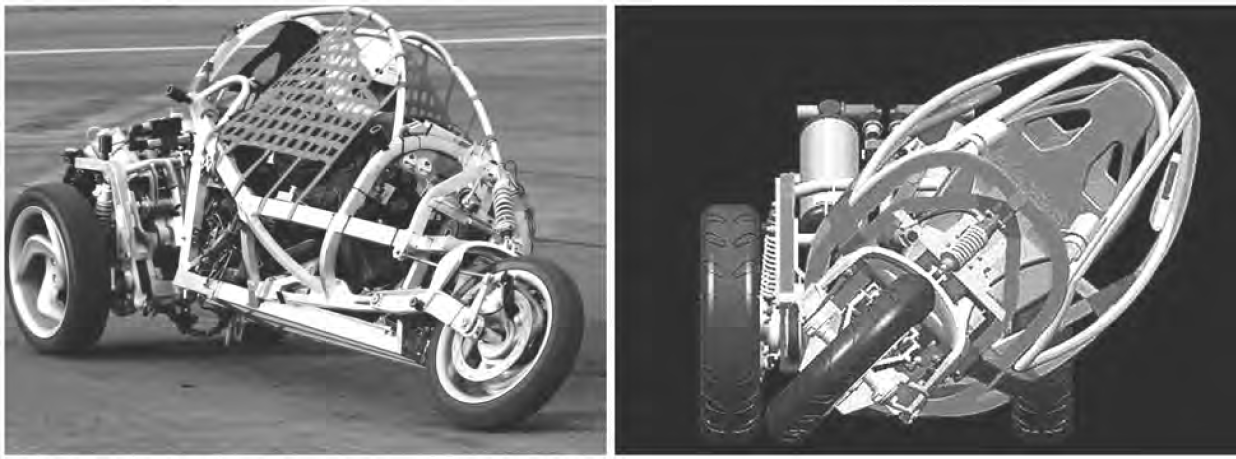
\includegraphics[width=.8\linewidth]{images/pt_02}
}%figues de la page de garde


\def\xxpied{%
Cycle 01 -- Modéliser le comportement des systèmes multiphysiques\\
Chapitre 2 -- \xxactivite%
}

\setcounter{secnumdepth}{5}
%---------------------------------------------------------------------------

\usepackage{pgfplots}
\begin{document}

%\chapterimage{png/Fond_Cin}
\pagestyle{empty}


%%%%%%%% PAGE DE GARDE COURS
\ifcours
% ==== BANDEAU DES TITRES ==== 
\begin{tikzpicture}[remember picture,overlay]
\node at (current page.north west)
{\begin{tikzpicture}[remember picture,overlay]
\node[anchor=north west,inner sep=0pt] at (0,0) {\includegraphics[width=\paperwidth]{\thechapterimage}};
\draw[anchor=west] (-2cm,-8cm) node [line width=2pt,rounded corners=15pt,draw=ocre,fill=white,fill opacity=0.6,inner sep=40pt]{\strut\makebox[22cm]{}};
\draw[anchor=west] (1cm,-8cm) node {\huge\sffamily\bfseries\color{black} %
\begin{minipage}{1cm}
\rotatebox{90}{\LARGE\sffamily\textsc{\color{ocre}\textbf{\xxnumpartie}}}
\end{minipage} \hfill
\begin{minipage}[c]{14cm}
\begin{titrepartie}
\begin{flushright}
\renewcommand{\baselinestretch}{1.1} 
\Large\sffamily\textsc{\textbf{\xxpartie}}
\renewcommand{\baselinestretch}{1} 
\end{flushright}
\end{titrepartie}
\end{minipage} \hfill
\begin{minipage}[c]{3.5cm}
{\large\sffamily\textsc{\textbf{\color{ocre} \discipline}}}
\end{minipage} 
 };
\end{tikzpicture}};
\end{tikzpicture}
% ==== FIN BANDEAU DES TITRES ==== 


% ==== ONGLET 
\begin{tikzpicture}[overlay]
\node[shape=rectangle, 
      rounded corners = .25 cm,
	  draw= ocre,
	  line width=2pt, 
	  fill = ocre!10,
	  minimum width  = 2.5cm,
	  minimum height = 3cm,] at (18.3cm,0) {};
\node at (17.7cm,0) {\rotatebox{90}{\textbf{\Large\color{ocre}{\classe}}}};
%{};
\end{tikzpicture}
% ==== FIN ONGLET 


\vspace{3.5cm}

\begin{tikzpicture}[remember picture,overlay]
\draw[anchor=west] (-2cm,-6cm) node {\huge\sffamily\bfseries\color{black} %
\begin{minipage}{2cm}
\begin{center}
\LARGE\sffamily\textsc{\color{ocre}\textbf{\xxactivite}}
\end{center}
\end{minipage} \hfill
\begin{minipage}[c]{15cm}
\begin{titrechapitre}
\renewcommand{\baselinestretch}{1.1} 
\Large\sffamily\textsc{\textbf{\xxnumchapitre}}

\Large\sffamily\textsc{\textbf{\xxchapitre}}
\vspace{.5cm}

\renewcommand{\baselinestretch}{1} 
\normalsize\normalfont
\xxcompetences
\end{titrechapitre}
\end{minipage}  };
\end{tikzpicture}
\vfill

\begin{flushright}
\begin{minipage}[c]{.3\linewidth}
\begin{center}
\xxfigures
\end{center}
\end{minipage}\hfill
\begin{minipage}[c]{.6\linewidth}
\startcontents
%\printcontents{}{1}{}
\printcontents{}{1}{}
\end{minipage}
\end{flushright}

\begin{tikzpicture}[remember picture,overlay]
\draw[anchor=west] (4.5cm,-.7cm) node {
\begin{minipage}[c]{.2\linewidth}
\begin{flushright}

\includegraphics[width=2cm]{logoCC}
\end{flushright}
\end{minipage}
\begin{minipage}[c]{.2\linewidth}
\textsl{\xxauteur} \\
\textsl{\classe}
\end{minipage}
 };
\end{tikzpicture}

\newpage
\pagestyle{fancy}

%\newpage
%\pagestyle{fancy}

\else
\fi
%% FIN PAGE DE GARDE DES COURS

%%%%%%%% PAGE DE GARDE TD
\iftd

% BANDEAU EXO
\iflivret % SI LIVRET
\begin{tikzpicture}[remember picture,overlay]
\draw[anchor=west] (-2cm,-3.3cm) node {\huge\sffamily\bfseries\color{black} %
\begin{minipage}{5cm}
\begin{center}
\LARGE\sffamily\color{ocre}\textbf{\textsc{\xxactivite}}

\begin{center}
\xxfigures
\end{center}

\end{center}
\end{minipage} \hfill
\begin{minipage}[c]{12cm}
\begin{titrechapitre}
\renewcommand{\baselinestretch}{1.1} 
\large\sffamily\textbf{\textsc{\xxtitreexo}}

\small\sffamily{\textbf{\textit{\color{black!70}\xxsourceexo}}}
\vspace{.5cm}

\renewcommand{\baselinestretch}{1} 
\normalsize\normalfont
\xxcompetences
\end{titrechapitre}
\end{minipage}};
\end{tikzpicture}
\else % ELSE NOT LIVRET
\begin{tikzpicture}[remember picture,overlay]
\draw[anchor=west] (-2cm,-4.5cm) node {\huge\sffamily\bfseries\color{black} %
\begin{minipage}{5cm}
\begin{center}
\LARGE\sffamily\color{ocre}\textbf{\textsc{\xxactivite}}

\begin{center}
\xxfigures
\end{center}

\end{center}
\end{minipage} \hfill
\begin{minipage}[c]{12cm}
\begin{titrechapitre}
\renewcommand{\baselinestretch}{1.1} 
\large\sffamily\textbf{\textsc{\xxtitreexo}}

\small\sffamily{\textbf{\textit{\color{black!70}\xxsourceexo}}}
\vspace{.5cm}

\renewcommand{\baselinestretch}{1} 
\normalsize\normalfont
\xxcompetences
\end{titrechapitre}
\end{minipage}};
\end{tikzpicture}

\fi

\else   % FIN IF TD
\fi


%%%%%%%% PAGE DE GARDE FICHE
\iffiche
\begin{tikzpicture}[remember picture,overlay]
\node at (current page.north west)
{\begin{tikzpicture}[remember picture,overlay]
\draw[anchor=west] (-2cm,-2.25cm) node [line width=2pt,rounded corners=15pt,draw=ocre,fill=white,fill opacity=0.6,inner sep=40pt]{\strut\makebox[22cm]{}};
\draw[anchor=west] (1cm,-2.25cm) node {\huge\sffamily\bfseries\color{black} %
\begin{minipage}{1cm}
\rotatebox{90}{\LARGE\sffamily\textsc{\color{ocre}\textbf{\xxnumpartie}}}
\end{minipage} \hfill
\begin{minipage}[c]{14cm}
\begin{titrepartie}
\begin{flushright}
\renewcommand{\baselinestretch}{1.1} 
\large\sffamily\textsc{\textbf{\xxpartie} \\} 

\vspace{.2cm}

\normalsize\sffamily\textsc{\textbf{\xxnumchapitre -- \xxchapitre}}
\renewcommand{\baselinestretch}{1} 
\end{flushright}
\end{titrepartie}
\end{minipage} \hfill
\begin{minipage}[c]{3.5cm}
{\large\sffamily\textsc{\textbf{\color{ocre} \discipline}}}
\end{minipage} 
 };
\end{tikzpicture}};
\end{tikzpicture}

\iflivret % SI LIVRET
\begin{tikzpicture}[overlay]
\node[shape=rectangle, 
      rounded corners = .25 cm,
	  draw= ocre,
	  line width=2pt, 
	  fill = ocre!10,
	  minimum width  = 2.5cm,
	  minimum height = 2.5cm,] at (18.5cm,.5cm) {};
\node at (17.9cm,.5cm) {\rotatebox{90}{\textsf{\textbf{\large\color{ocre}{\classe}}}}};
%{};
\end{tikzpicture}
\else  % SI PAS LIVRET
\iftd %% SI TD et PAS LIVRET
\begin{tikzpicture}[overlay]
\node[shape=rectangle, 
      rounded corners = .25 cm,
	  draw= ocre,
	  line width=2pt, 
	  fill = ocre!10,
	  minimum width  = 2.5cm,
	  minimum height = 2.5cm,] at (18.6cm,0.9cm) {};
\node at (18cm,0.9cm) {\rotatebox{90}{\textsf{\textbf{\large\color{ocre}{\classe}}}}};
%{};
\end{tikzpicture}

\else % FIN DU SI TD PAS LIVRET 
\begin{tikzpicture}[overlay]
\node[shape=rectangle, 
      rounded corners = .25 cm,
	  draw= ocre,
	  line width=2pt, 
	  fill = ocre!10,
	  minimum width  = 2.5cm,
%	  minimum height = 2.5cm,] at (18.5cm,1.1cm) {};
	  minimum height = 2.5cm,] at (18.6cm,0.5cm) {};
\node at (18cm,0.5cm) {\rotatebox{90}{\textsf{\textbf{\large\color{ocre}{\classe}}}}};
%{};
\end{tikzpicture}
\fi
\fi
\else
\fi



\vspace{4.5cm}
\pagestyle{fancy}
\thispagestyle{plain}

\def\columnseprulecolor{\color{ocre}}
\setlength{\columnseprule}{0.4pt} 

\def\pathfig{images}

\begin{multicols}{2}
%\subsection*{Mise en situation}

%\section{Véhicule à 3 roues Clever}
\subsection*{Mise en situation}

Le Clever, présenté sur la Figure 1, est un démonstrateur technologique développé par un tissu d'industriels européens -- dont BMW, l'Institut Français du Pétrole (IFP) et de nombreux équipementiers -- grâce au financement de l'Union Européenne. Clever est la contraction de Compact Low Emission VEhiclefor uRban tRansportation (véhicule compacte à faibles émissions pour le transport urbain) car, avec une consommation de seulement \SI{2,5}{L/100 km}, il s'annonce très écologique. Les premiers prototypes ont vu le jour en 2006. Ce type de véhicule pourrait être un des prochains commercialisés par BMW si le prix de vente peut être ramené sous la barre des 10 000 euros.

    

\begin{center}
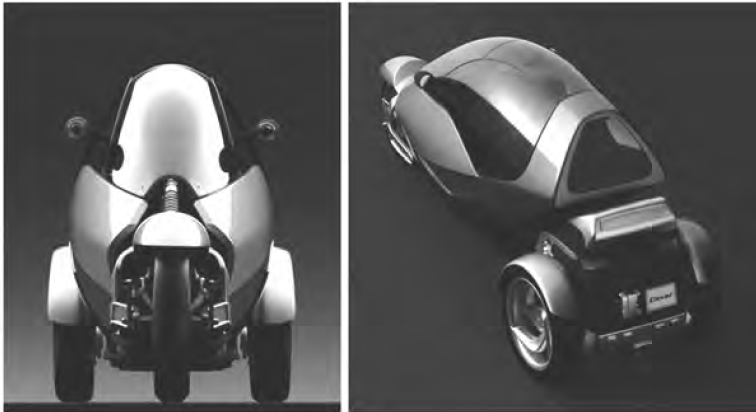
\includegraphics[width=.5\linewidth]{images/pt_01_Bis}

\textit{Figure 1 --Véhicule à trois roues Clever}
\end{center} 



%La Figure 2 présente un diagramme partiel des interacteurs, issu de l'analyse fonctionnelle du besoin dans la phase d'utilisation normale (véhicule Clever utilisé pour se déplacer). %Le Tableau 1 décrit les fonctions de service correspondantes. 
%À l'issue de l'analyse fonctionnelle technique, les solutions qui ont été retenues sont les suivantes : le Clever se présente comme un véhicule à trois roues pouvant embarquer deux personnes assises en tandem. Il adopte une architecture pendulaire, c'est-à-dire qu'il se penche dans les virages (cf. Figure 2). Le déplacement du centre de gravité qui en résulte lui confère une grande stabilité malgré une faible largeur du véhicule (légèrement inférieure à \SI{1}{m}, contre 60 à \SI{75}{cm} pour une moto, et \SI{1,5}{m} pour une petite voiture). Cette étroitesse se veut une réponse aux problèmes d'encombrement dans les villes mais permet aussi une surface frontale moins importante que sur une voiture conventionnelle et donc des pertes aérodynamiques réduites. En outre, les sensations de conduite sont semblables à celle d'une moto mais avec un pilotage, à l'aide d'un volant, propre à un véhicule à 4 roues. Le moteur est un monocylindre à gaz naturel qui a été développé par l'IFP et dont les performances permettent d'atteindre une vitesse de pointe de \SI{100}{km.h^{-1}} avec une accélération en phase avec les attentes pour un véhicule urbain.


%
%\begin{center}
%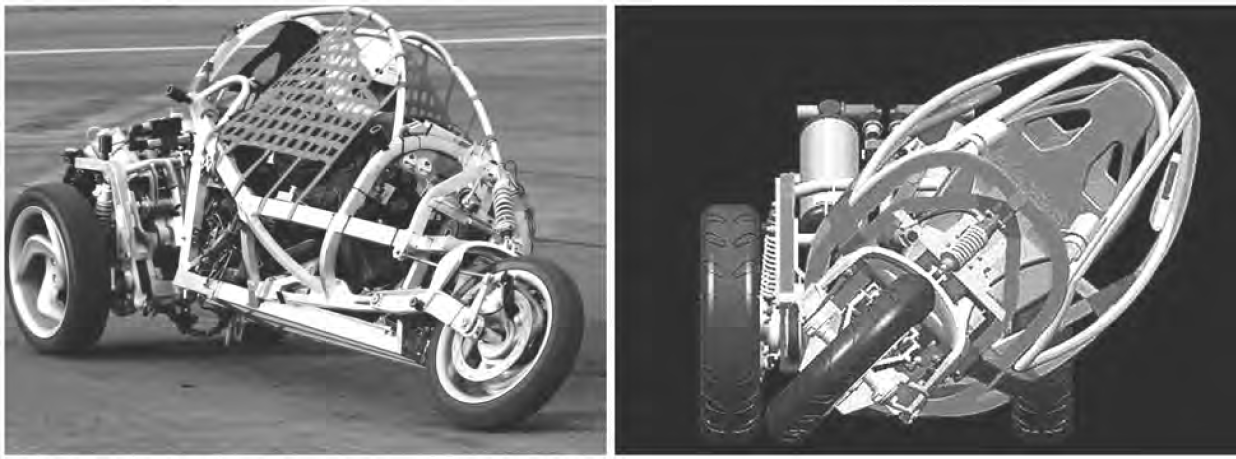
\includegraphics[width=.5\linewidth]{images/pt_02}
%
%\textit{Figure 2 --Vue de la cinématique pendulaire }
%\end{center} 


\subsection*{Validation des critères principaux de la fonction technique «~Transmettre la puissance mécanique~»}

\begin{obj}
L'objectif de cette partie est de vérifier l'aptitude de la chaine d'énergie choisie par le constructeur à valider certains critères de la fonction technique « Transmettre la puissance mécanique » qui a été proposée pour assurer la fonction technique FT1 « Modifier l'inclinaison de l'habitacle ». Pour cela, on mettra en place un modèle de comportement suffisamment pertinent pour appréhender les caractéristiques principales du comportement du système réel.
\end{obj}


 \begin{center}
 \begin{tabular}{|p{2.5cm}|p{2.5cm}|p{2.5cm}|}
 \hline
 Fonction technique & Critères d'appréciation	& Niveau \\ \hline
\multirow{2}{2.5cm}{Transmettre la puissance mécanique}
& Amplitude de mouvement &  $- 45\degres$ à $+ 45\degres$ \\ \cline{2-3}
& Vitesse de rotation & de $- 45\degres$ à $+ 45\degres$ en \SI{1,5}{s} \\ 
 \hline
\multirow{4}{2.5cm}{Contrôler le mouvement de l'habitacle} & & \\
& Écart statique & nul \\ \cline{2-3}
& Écart de traînage &  0\degres \\ \cline{2-3}
& Temps de réponse à 5\% & $\leq$ \SI{0,1}{s} \\ \cline{2-3}
& Marge de phase & comprise entre 45\degres et 50\degres \\
  \hline
 \end{tabular}
 \end{center}
 
 
\subsubsection*{Description du système d'inclinaison de l'habitacle}
Le système d'inclinaison de l'habitacle est assuré par un système constitué :
\begin{itemize}
\item d'un calculateur qui détermine le mouvement et la position à donner à l'habitacle en fonction des conditions d'utilisation ;
\item d'un système hydro-mécanique de transmission de puissance et d'adaptation de mouvement ;
\item d'un système de contrôle de l'inclinaison de l'habitacle.
\end{itemize}

La chaîne de transmission de puissance et d'adaptation de mouvement est composée (Figure II.1) :
\begin{itemize}
\item d'une pompe à engrenages actionnée par le moteur à gaz via un système de poulies/courroie ;
\item d'un circuit hydraulique ;
\item de 2 vérins hydrauliques simple effet ;
\item d'un système mécanique d'adaptation de mouvement afin de transformer le mouvement de translation des tiges des vérins en rotation de l'habitacle.
\end{itemize}

\begin{center}
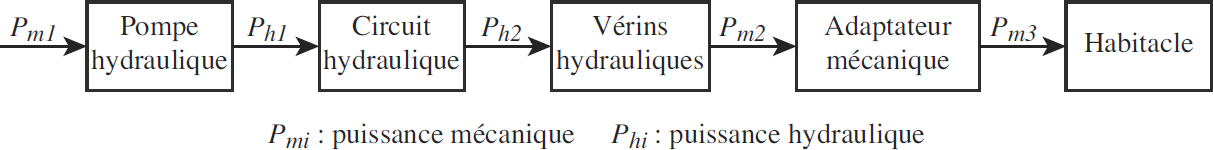
\includegraphics[width=\linewidth]{images/pt_03}

\textit{Figure II.1 - Chaîne de transmission de puissance}
\end{center}


Les deux vérins hydrauliques transforment la puissance hydraulique venant du servo-distributeur afin d'incliner l'habitacle. Ceux-ci sont disposés entre l'habitacle et le châssis du module arrière de propulsion. Le calculateur autorise ou non, l'alimentation en huile de l'un des vérins provoquant la sortie de tige, pendant que l'huile s'évacue de l'autre vérin. Ainsi l'habitacle s'incline du coté opposé au vérin alimenté. Lorsque l'habitacle est en position centrale, les tiges de vérin sont en position médiane.


\subsubsection*{Détermination du gain statique du servo-distributeur}
L'orientation de l'habitacle est contrôlée par un asservissement de la position angulaire. L'architecture de cet asservissement est représentée par le schéma-bloc de la Figure II.3.

Le temps de réponse du servo-distributeur est suffisamment faible pour que l'on puisse modéliser son comportement par un gain pur noté $K_s$. Le comportement du capteur est supposé linéaire dans la gamme d'utilisation qui nous intéresse ici. On pose : $H_c(p) = C$ avec      $ C = \SI{1}{V/rad}$.

À ce stade de l'étude, le modèle de comportement du fluide correspond à un comportement incompressible. L'équation caractérisant le comportement du vérin est alors : $q(t)=S\dot{\lambda}(t)$ où :
\begin{itemize}
\item $S$ représente la section utile du vérin en sortie de tige (diamètre \SI{32}{mm});
\item $q$ est le débit en entrée de vérin ;
\item $\dot{\lambda}(t)=\dfrac{\dd \lambda(t) }{\dd t}$ est la vitesse de translation de la tige du vérin par rapport au corps.
\end{itemize}


\begin{center}
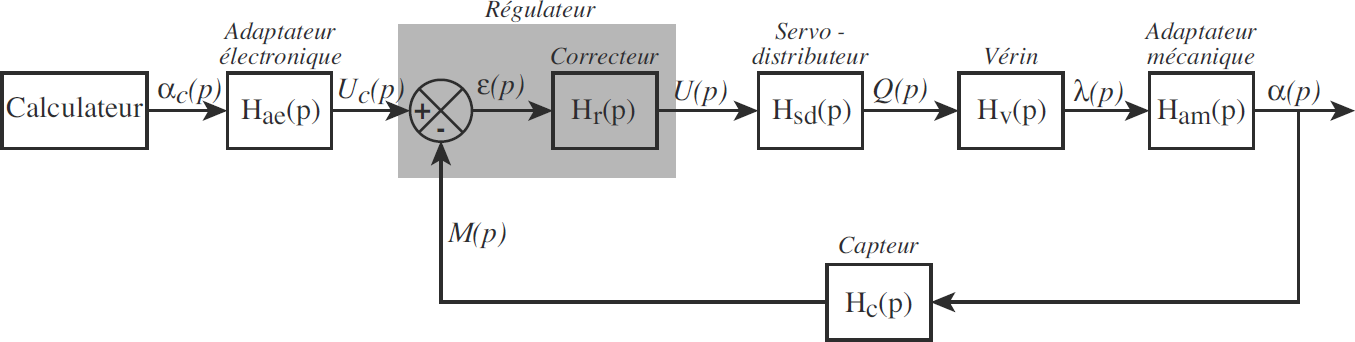
\includegraphics[width=.9\linewidth]{images/pt_05}

\textit{Figure II.3 – Architecture générale du contrôle de l’orientation de l’habitacle}
\end{center}

%\subsubsection{Détermination de la loi entrée/sortie géométrique de l'adaptateur mécanique}
%On suppose que le mécanisme étudié admet  $\left(O,\vect{z_0},\vect{x_0} \right)$ comme plan d'étude. Le modèle cinématique adopté est précisé par le schéma cinématique de la Figure II.4, sur laquelle sont aussi représentées les données géométriques et les paramètres de mouvements qui seront utilisés dans la question suivante afin de simplifier l'étude.
%
%
%
%\begin{center}
%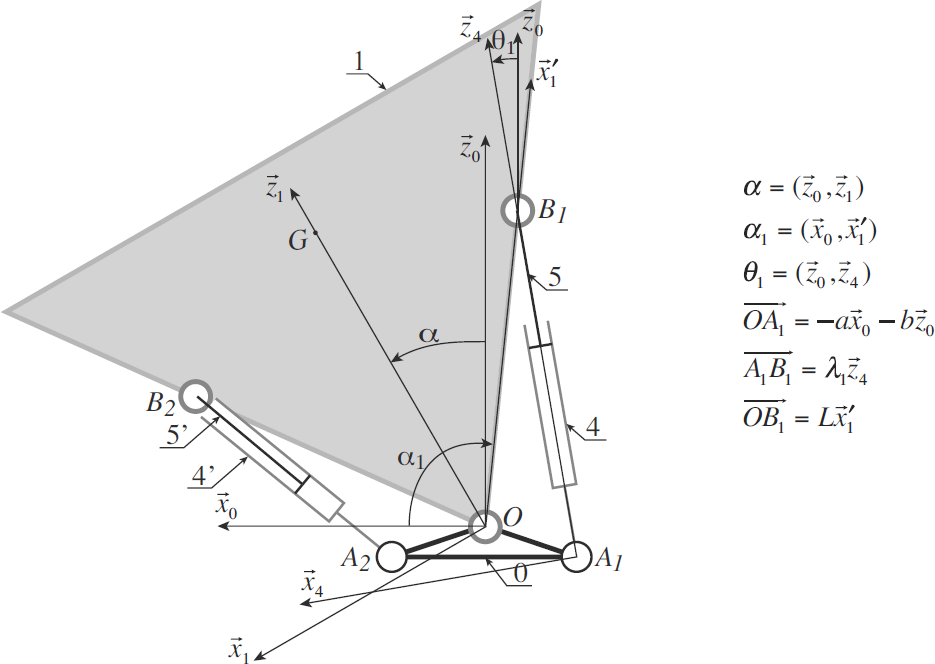
\includegraphics[width=.8\linewidth]{images/pt_04}
%
%\textit{Figure II.4 - Paramétrage cinématique adopté pour l'étude analytique}
%\end{center}
%
%
%\subparagraph{}
%\textit{Déterminer 2 équations scalaires reliant $\alpha_1$ (on a $\alpha=\alpha_1-\alpha_{10}$, avec $\alpha_{10}$ valeur de $\alpha_{1}$ pour l'habitacle non-incliné), $\theta_1$ et $\lambda_1$ (les directions de projection seront judicieusement choisies). En éliminant le paramètre $\theta_1$, mettre la relation entre $\alpha_{1}$ et $\lambda_1$ sous la forme :
%$\cos\left(\alpha_1+\psi\right)=\dfrac{A}{B}$ en précisant les expressions de $\psi$, $A$ et $B$ en fonction de $a$, $b$, $L$ et $\lambda_1$.}
%\ifprof
%\begin{corrige}
%\end{corrige}
%\else
%\fi
%
%
%Le tracé de cette relation est laborieux sans moyen numérique. Aussi, il vous est proposé de déterminer la position de
%certains points de la courbe $\alpha\left( \lambda_1 \right)$ en prenant 2 positions d'inclinaison de l'habitacle entre 0 et
%45\degres. On obtient ainsi 7 points pour la plage de variation de $\alpha$ (de $- 45\degres$ à $45\degres$). Pour cela,
%on adopte le paramétrage de la Figure II.4 en prenant comme origine des angles la position 
%<< habitacle non-incliné >>.
%
%\subparagraph{}
%\textit{Représenter sur la figure du Cahier Réponses les positions des points $B_1$ et $B_2$ pour les 2 positions angulaires choisies. Tracer l'évolution de $\alpha$ en fonction de $\lambda_1$ pour $\alpha$ compris entre $- 45\degres$ et $+ 45\degres$. Est-il possible de décrire cette courbe par une fonction linéaire en prenant comme origine les valeurs des paramètres pour la position << habitacle non-incliné >> (on définit alors le paramètre $\lambda$ tel que : $\lambda = \lambda_1 - \lambda_{10}$) ? Si oui, donner une valeur approximative de sa pente, paramètre noté $R$ pour la suite.}
%\ifprof
%\begin{corrige}
%\end{corrige}
%\else
%\fi


\subsubsection*{Détermination du gain du servo-distributeur}

On considère le schéma-bloc du Cahier Réponses.

\subparagraph{}\textit{Donner l'expression de la fonction de transfert du vérin $H_{V1}(p)$ (telle que $\lambda(p) = H_{V1}(p) Q(p)$). Proposer une fonction de transfert de l'adaptateur électroniquer $H_{ae}(p)$ afin d'assurer l'asservissement angulaire de l'habitacle. Compléter le schéma-bloc associé à la modélisation actuelle du système.}
\ifprof
\begin{corrige}
\end{corrige}
\else
\fi


\subparagraph{}\textit{Déterminer la fonction de transfert en boucle fermée $\text{FTBF}_1$ (telle que $\alpha(p) = \text{FTBF}_1(p) \alpha_c(p)$) du système bouclé. Mettre  $\text{FTBF}_1(p)$ sous la forme 
$\dfrac{K_1}{1+\tau_1 p}$ en précisant les expressions de $K_1$ et de $\tau_1$.} 
\ifprof
\begin{corrige}
\end{corrige}
\else
\fi


\subparagraph{}\textit{ À partir du critère de temps de réponse à 5\% $(t_{r5\%})$ du système, déterminer l'expression puis la valeur numérique minimale du gain du servo-distributeur.} 
\ifprof
\begin{corrige}
\end{corrige}
\else
\fi



\subsubsection*{Analyse des caractéristiques prévues par le modèle}

On cherche ici à déterminer les caractéristiques de la régulation de la position angulaire de l'habitacle prévu par le modèle construit précédemment.

\subparagraph{}\textit{ Déterminer l'écart de traînage $\varepsilon_{\text{tr}}$ prévu par le modèle actuel. Le critère de précision statique est-il satisfait ?} 
\ifprof
\begin{corrige}
\end{corrige}
\else
\fi


On place un intégrateur dans le régulateur. On a alors : $H_r(p)=\dfrac{1}{p}$.
 

\subparagraph{}\textit{La précision statique et l'écart de traînage sont-il satisfaits ?} 
\ifprof
\begin{corrige}
\end{corrige}
\else
\fi

\subparagraph{}\textit{ Donner la valeur de la marge de phase. Conclure.} 
\ifprof
\begin{corrige}
\end{corrige}
\else
\fi

\subsection*{Modélisation du comportement dynamique}

L'hypothèse d'incompressibilité formulée dans la partie précédente conduit à un modèle purement cinématique qui ne tient pas compte des effets dynamiques. On choisit d'utiliser un modèle de fluide compressible pour affiner l'analyse du comportement dynamique. L'étude est réalisée en considérant le véhicule Clever à l'arrêt en vue d'effectuer des premiers tests.


\subsubsection*{Modélisation du comportement du vérin avec fluide compressible}

La compressibilité du fluide étant prise en compte dans le modèle, l'évolution du débit est une fonction du déplacement mais aussi de la pression sous la forme de la relation (1). L'effort exercé par le vérin en sortie de tige est décrit par la relation (2).

$$
q(t)=S\dot{\lambda}(t)+\dfrac{V_0}{B}\dot{p}_r(t) \quad (1) \quad\quad
F_V(t)=Sp_r(t) \quad (2)
$$
où:
\begin{itemize}
\item $p_r(t)$ : pression utile dans le vérin ;
\item $V_0$ : volume caractéristique moyen de fluide contenu dans le vérin et les durites, $V_0 = \SI{2,5e5}{m^3}$;
\item $B$ : coefficient de compressibilité du fluide, $B = \SI{109}{Pa}$;
\item $F_v(t)$ : effort développé par le vérin en sortie de tige ;
\item $S$ : section utile du vérin en sortie de tige.
\end{itemize}

On a de plus $F_v(t)+k_g \lambda(t)=m_{\text{eq}}\ddot{\lambda}(t)$ avec $m_{\text{eq}}$ la masse équivalente du système, $k_g$ une constante, $\lambda(t)$ le déploiement des vérins.



\subparagraph{}\textit{Appliquer la transformation de Laplace aux équations précédentes et compléter le schéma-blocs.}
\ifprof
\begin{corrige}
\end{corrige}
\else
\fi


\subsubsection*{Analyse du comportement global}

\begin{obj}
L’objectif de cette partie est d’analyser le comportement décrit par le modèle de fluide compressible. Afin de
valider le modèle établi, on se propose d’étudier le comportement en boucle fermée de la chaîne fonctionnelle de
commande du vérin.
\end{obj}






\subparagraph{}
\textit{Donner l’expression de la fonction de transfert en boucle fermée du vérin $H_{V2}$ (telle que $\lambda(p) =
H_{V2}(p) Q(p)$ ) et préciser les expressions des coefficients $K_V$ et $\omega_V$ de sa forme canonique :
$H_{V2}(p)=\dfrac{K_V}{p\left( 1+\dfrac{p^2}{\omega_V^2}\right)}$.}
\ifprof
\begin{corrige}
\end{corrige}
\else
\fi



\subparagraph{}
\textit{Montrer à partir des valeurs numériques des termes de $\omega_V$ et de $K_V$ que le terme $k_g$ peut être
négligée (on rappelle : $e = \SI{0.5}{m}$). Ceci revient à enlever le bloc associé à ce paramètre du schéma-blocs. On conservera cette simplification dans toute la suite du sujet.}
\ifprof
\begin{corrige}
\end{corrige}
\else
\fi




\subsubsection*{Modélisation du comportement dynamique avec prise en compte d'un débit de fuite}
Pour pallier le problème de stabilité du modèle précédemment établi, une solution possible consiste à introduire un débit de fuite au niveau du vérin. Celui-ci a pour effet de réduire artificiellement le débit réel entrant dans le vérin en fonction de la pression utile. L'expression du débit est alors : 
$q(t)=S\dot{\lambda}(t)+\dfrac{V_0}{B} \dot{p}_r(t)-\delta p_r(t)$ où $\delta$ représente le coefficient de débit de fuite.


\subparagraph{}\textit{Proposer une modification du schéma-blocs donné afin de prendre en compte le débit de fuite.}
\ifprof
\begin{corrige}
\begin{center}
%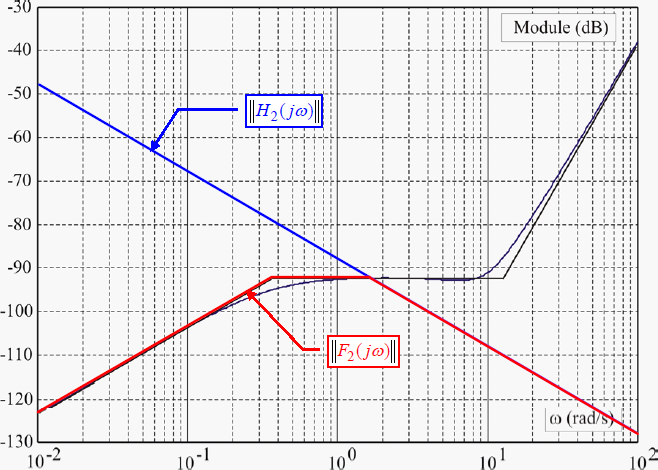
\includegraphics[width=.95\linewidth]{images/cor_07}
%\textit{}
\end{center}
\end{corrige}
\else
\fi
\begin{center}
%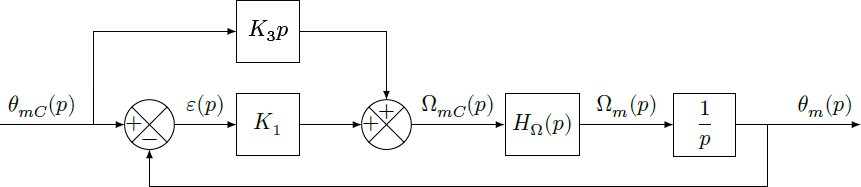
\includegraphics[width=\linewidth]{images/fig_08}
%\textit{}
\end{center}


\subparagraph{}\textit{Déterminer l'expression de la fonction de transfert $H_{V3}$ (telle que $\lambda(p) =  H_{V3} Q(p)$) associée au comportement dynamique du vérin ainsi modélisé. On donnera le résultat sous la forme suivante : 
$H_{V3}(p)=\dfrac{K_V}{p\left(1+a_1 p + \dfrac{p^2}{\omega_V^2} \right)}$.  
Donner l'expression de $a_1$ en fonction de $M_{\text{eq}}$, $\delta$ et $S$ et déterminer l'expression du coefficient d'amortissement $\xi_V$ du second ordre en fonction de $M_{\text{eq}}$, $\delta$, $S$, $B$ et $V_0$.}
\ifprof
\begin{corrige}
\begin{center}
%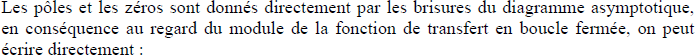
\includegraphics[width=.95\linewidth]{images/cor_08}
%\textit{}
\end{center}
\end{corrige}
\else
\fi

\subsubsection*{Analyse du comportement global et détermination de la valeur limite du coefficient de débit de fuite}


L'objectif de cette partie est d'analyser le comportement dynamique prévu par le modèle développé précédemment. Pour cela, on considère le système modélisé par le schéma bloc de la Figure II.3.

\subparagraph{}\textit{Déterminer la valeur numérique de $\omega_V$.}
\ifprof
\begin{corrige}
\end{corrige}
\else
\fi


Quels que soient les résultats obtenus précédemment, on prendra les valeurs numériques suivantes :

$$C = \SI{1}{V/rad} \quad\quad K_S = \SI{65e-4}{m^3.s^{-1}.V^{-1}} \quad\quad  K_V = \SI{1,25e3}{m^{-2}.s}\quad\quad  R = \SI{7,5}{rad/m}.$$


\subparagraph{}\textit{Tracer le diagramme asymptotique de Bode de la fonction de transfert en boucle ouverte FTBO1 du système asservi, avec : $M(p)=\text{FTBO}_1(p) \varepsilon(p)$.}
\ifprof
\begin{corrige}
\end{corrige}
\else
\fi

\subparagraph{}\textit{Déterminer la valeur limite de $\xi_V$ assurant la stabilité du modèle. À partir de l'expression de $\xi_V$ déterminer la valeur numérique limite du coefficient de débit de fuite $\delta$.}

\ifprof
\begin{corrige}
\end{corrige}
\else
\fi



\subsection*{Validation des critères principaux de la fonction technique <<~Contrôler le mouvement de l'habitacle~>> }

\begin{obj}
L'objectif de cette partie est de définir le correcteur et de déterminer les valeurs numériques de ses paramètres caractéristiques, afin d'obtenir un asservissement en poursuite du mouvement de l'habitacle validant les critères de la fonction technique FT13 <<~Contrôler le mouvement de l'habitacle~>> qui a été proposée pour assurer la fonction technique FT1 <<~Modifier l'inclinaison de l'habitacle~>>.
\end{obj}

\subsubsection*{Synthèse des résultats obtenus précédemment}


On considère le schéma-blocs de la figure III.1 avec :
$$
H_C(p)=C \quad \quad H_{sd}(p)=K_S \quad \quad H_{am}(p)=R \quad \quad  H_{V}(p)=\dfrac{K_V}{p\left(1+ 2\dfrac{\xi_V}{\omega_V}p + \dfrac{p^2}{\omega_V^2} \right)}
$$


\begin{center}
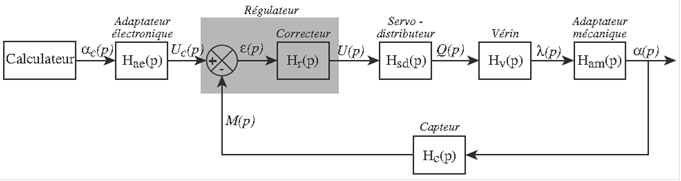
\includegraphics[width=.9\linewidth]{images/pt_06}

\textit{Figure III.1 - Architecture générale du contrôle de l'orientation de l'habitacle}
\end{center}

Quels que soient les résultats obtenus précédemment, on prendra les valeurs numériques suivantes :
$$C = \SI{1}{V/rad} \quad\quad K_S = \SI{3e-3}{m^3.s^{-1}.V^{-1}} \quad\quad  K_V = \SI{1,25e3}{m^{-2}.s}\quad\quad  R = \SI{7,5}{rad/m} \quad \quad  \omega_V=\SI{50}{rad.s^{-1}}    \quad \quad  \xi_V = 0,5.$$


Le temps de réponse de l'adaptateur électronique est suffisamment faible comparativement aux temps caractéristiques des autres systèmes pour que l'on puisse modéliser son comportement temporel par un gain pur $K_{\text{ae}}$.

\subparagraph{}
\textit{Donner l'expression de $K_{\text{ae}}$ pour que l'écart $\varepsilon(t)$ ait un sens.}
\ifprof
\begin{corrige}
\end{corrige}
\else
\fi

\subsection*{Première correction}
Afin de répondre au critère du cahier des charges concernant la précision statique du système, on choisit de placer un intégrateur comme premier correcteur : $H_r(p)=\dfrac{K_i}{p}$.

\subparagraph{}
\textit{On donne sur le Cahier Réponses le diagramme de Bode de la fonction de transfert en boucle ouverte $ \text{FTBO}_2(p)$ du système asservi pour $K_i = 1$ et telle que $M(p) = \text{FTBO}_2(p).\varepsilon(p)$. Déterminer, en expliquant clairement la méthode employée, la valeur de $K_i$ qui permet d'obtenir la dynamique souhaitée.}
\ifprof
\begin{corrige}
\end{corrige}
\else
\fi

On donne en annexe page 8 la définition d'un correcteur à avance de phase.
\subparagraph{}
\textit{Combien de correcteurs à avance de phase réglés pour apporter chacun 50\degres au maximum faudrait-il incorporer dans le régulateur pour satisfaire le critère de marge de phase du cahier des charges ?}
\ifprof
\begin{corrige}
\end{corrige}
\else
\fi



On souhaite réaliser une simulation du comportement temporel du système ainsi corrigé pour un passage de 0 à 45\degres de l'habitacle en \SI{0,75}{s}. Le signal de consigne est donné sur la Figure III.2. Le logiciel de simulation ne possède pas de bloc de signal d'entrée correspondant à ce type de fonction, mais il est possible d'utiliser des blocs de type  <<~rampe~>> possédant les critères :
\begin{itemize}
\item pente de la rampe ;
\item instant de départ de la rampe.
\end{itemize}


\begin{center}
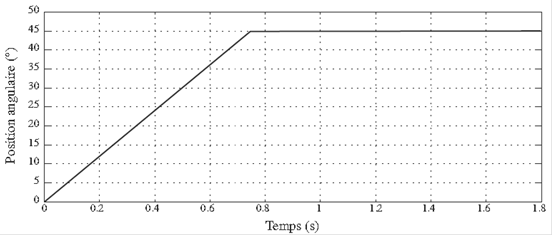
\includegraphics[width=.6\linewidth]{images/pt_07} 

\textit{Figure III.2 - Signal de consigne pour une simulation d'une rotation de 0 à 45\degres en \SI{0,75}{s}}
\end{center}



\subparagraph{}
\textit{Donner les paramètres à entrer dans les 2 blocs de type << rampes >> et préciser l'opération mathématique à effectuer entre les deux blocs afin d'obtenir le signal présenté sur la Figure III.2.}
\ifprof
\begin{corrige}
\end{corrige}
\else
\fi

La réponse obtenue par la simulation est présentée sur la Figure III.3.

\subparagraph{}
\textit{Quels sont les critères non satisfaits ?}
\ifprof
\begin{corrige}
\end{corrige}
\else
\fi



\begin{center}
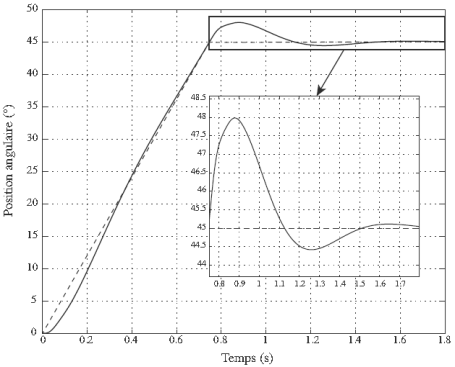
\includegraphics[width=.5\linewidth]{images/pt_08} 

\textit{Figure III.3 - Résultat de la simulation du passage de de 0 à 45\degres en \SI{0,75}{s}}
\end{center}


\subsection*{Deuxième correction}

Plusieurs réglages du correcteur précédent ont été réalisés mais aucun n'a pu apporter satisfaction quant aux différents critères du cahier des charges. Le problème de fond ici est lié au fait que la pulsation de coupure $\omega_V$ du mode de second ordre de la fonction de transfert du vérin est inférieure à la pulsation à \SI{0}{dB} souhaitée pour garantir une dynamique suffisante du système bouclé. On souhaite donc augmenter la valeur de la pulsation de coupure $\omega_V$ afin de garantir au moins deux décades d'écart avec la pulsation à 0 dB de la fonction de transfert en boucle ouverte du système.

\subparagraph{}
\textit{Quelle valeur de diamètre du vérin permet de vérifier la condition précédente. Cette valeur est-elle réaliste ?}
\ifprof
\begin{corrige}
\end{corrige}
\else
\fi


On décide alors de remédier à ce problème par un filtre électronique du second ordre de type Notch de fonction de transfert :

$H_{N}(p)=\dfrac{1+ \dfrac{2\xi_n}{\omega_n}p + \dfrac{p^2}{\omega_n^2} }{1+ \dfrac{2\xi_d}{\omega_d}p + \dfrac{p^2}{\omega_d^2} }$.

Le réglage optimum du correcteur doit compenser parfaitement le mode de second ordre de la fonction de transfert du vérin. Pour cela, on effectue un essai afin d'identifier les caractéristiques de ce mode. Aucun réglage spécifique du débit de fuite n'a été réalisé, la compensation du mode rendant inutile cette étape.

Une tension de consigne $u_e(t) = 0,02u(t)$ (avec $u(t)$ l'échelon unitaire) est envoyée en entrée du servo-distributeur. Une génératrice tachymétrique, dont le comportement est modélisé par un gain pur $K_{\text{gt}} = \SI{2}{V.rad^{-1}.s}$, mesure la vitesse de rotation de l'habitacle. Cette tension est notée $m_{\omega}(t)$. Le résultat de cet essai est donné sur la Figure de la question 24 du Cahier Réponses.


\subparagraph{}
\textit{Compléter sur le Cahier Réponses le schéma-blocs représentant cet essai et déterminer la fonction de transfert $H_{\text{essai}}$ telle que : $M_{\Omega}(p) = H_{\text{essai}}(p)U_e(p)$.}
\ifprof
\begin{corrige}
\end{corrige}
\else
\fi


 
\subparagraph{}
\textit{En vous aidant du graphe de la Figure III.4, déterminer les valeurs numériques expérimentales de $\omega_v$ et 
$\xi_v$ à partir de la courbe obtenue expérimentalement tracée sur le Cahier Réponses.}
\ifprof
\begin{corrige}
\end{corrige}
\else
\fi

\subparagraph{}
\textit{Quels inconvénients sur le comportement réel du système peuvent découler de cette méthode consistant à vouloir compenser le mode de second ordre de la fonction de transfert du vérin par ce type de filtre électronique ?}
\ifprof
\begin{corrige}
\end{corrige}
\else
\fi

\begin{center}
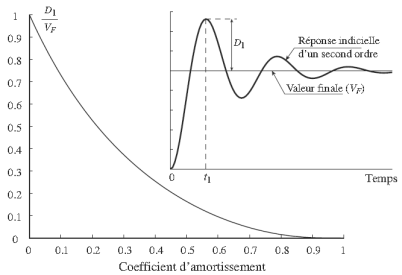
\includegraphics[width=.6\linewidth]{images/pt_09}

\textit{Figure III.4 - Évolution du premier dépassement relatif à la valeur finale en fonction du coefficient d'amortissement (pour une fonction de transfert du second ordre)}
\end{center}

On suppose par la suite que le numérateur du filtre Notch compense parfaitement le mode de second ordre de la fonction de transfert du vérin. On adopte les caractéristiques suivantes pour le dénominateur :
\begin{itemize}
\item $\omega_d = \SI{1000}{rad.s^{-1}}$ ;
\item $\xi_d = 1$.
\end{itemize}

Afin de satisfaire le critère de précision statique du cahier des charges on place un premier correcteur de type intégrateur non unitaire de fonction de transfert :
$H_{\text{cor2}}(p)=\dfrac{K_{\Omega}}{p}$.

La valeur de $K_{\Omega}$ est déterminée afin d'obtenir une pulsation à \SI{0}{dB} de la fonction de transfert en boucle ouverte de \SI{65}{rad.s^{-1}}. Le diagramme de Bode de cette fonction de transfert est donné sur la Figure III.5.
On complète le régulateur par un correcteur à avance de phase de fonction de transfert :
$H_{\text{av}}(p)=K_{\text{av}}\dfrac{1+a_{\text{av}}\tau_{\text{av}}p}{1+\tau_{\text{av}}p}$ avec $a_{\text{av}}>1$.

On donne en annexe page 8 la définition d'un correcteur à avance de phase.

\subparagraph{}
\textit{Déterminer les valeurs approximatives des paramètres $a_{\text{av}}$, $\tau_{\text{av}}$ et $K_{\text{av}}$ qui permettent de satisfaire le critère de marge de phase du cahier des charges tout en conservant une pulsation à \SI{0}{dB} de \SI{65}{rad.s^{-1}}.}
\ifprof
\begin{corrige}
\end{corrige}
\else
\fi



Le régulateur étant a priori optimisé, on réalise un essai de validation du comportement temporel de l'inclinaison de l'habitacle, le véhicule étant à l'arrêt. Le calculateur envoie un signal de consigne représentant l'évolution de la position angulaire souhaitée (de 0 à 45\degres en \SI{0,75}{s}). La tension délivrée par le capteur angulaire est récupérée par un convertisseur analogique-numérique afin de tracer sur un ordinateur l'évolution temporelle de l'inclinaison de l'habitacle mesurée en degrés. Les deux courbes sont données sur la Figure III.6.


\subparagraph{}
\textit{Quels sont les critères du cahier des charges validés ?}


\begin{minipage}[c]{.48\linewidth}
\begin{center}
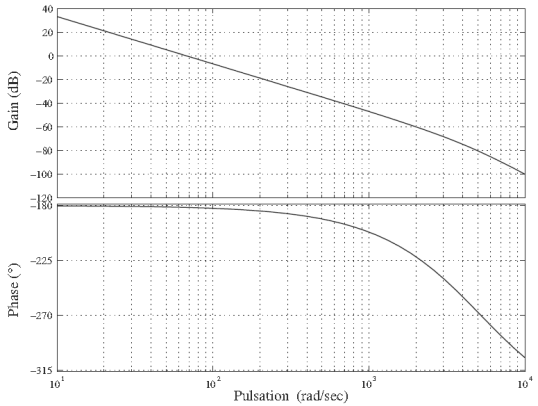
\includegraphics[width=.95\linewidth]{images/pt_10}

\textit{Figure III.5 - Diagramme de Bode de la Fonction de Transfert en Boucle Ouverte après correction Intégrale}
\end{center}
\end{minipage} \hfill
\begin{minipage}[c]{.48\linewidth}
\begin{center}
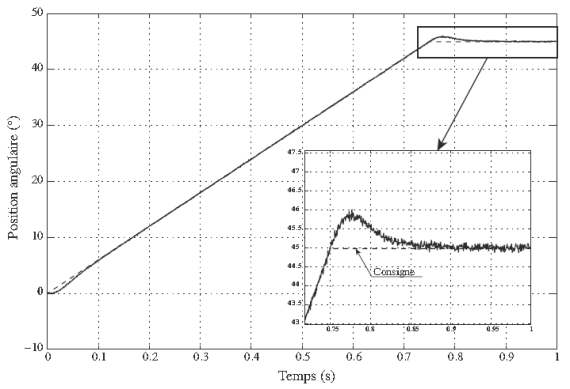
\includegraphics[width=.95\linewidth]{images/pt_11}

\textit{Figure III.6 - Essai de validation : passage de 0 à 45\degres \, en  \SI{0,75}{s}}
\end{center}
\end{minipage}








\section*{Annexe : Caractéristiques fréquentielles d’un correcteur à avance de phase}
 


\begin{minipage}[c]{.4\linewidth}
Sur la figure sont précisés les diagrammes de Bode d'un correcteur à avance de phase de fonction de transfert :
$H_{\text{av}}(p)=K_{\text{av}}\dfrac{1+a_{\text{av}}\tau_{\text{av}}p}{1+\tau_{\text{av}}p}$ avec $a_{\text{av}}>1$.


La phase maximum $\varphi_m$ est reliée au paramètre $a_{\text{av}}$ par la relation suivante : $\varphi_m=\dfrac{a_{\text{av}}-1}{a_{\text{av}}+1}$.
\end{minipage} \hfill
\begin{minipage}[c]{.58\linewidth}
\begin{center}
%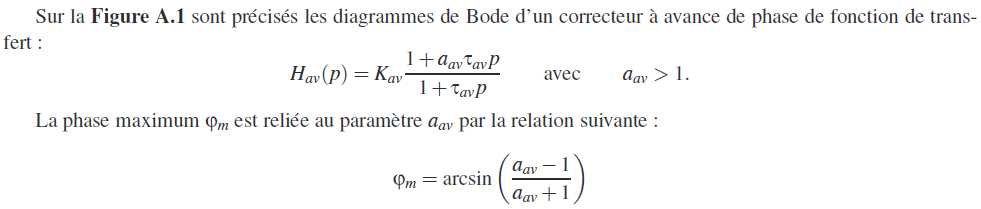
\includegraphics[width=\linewidth]{images/pt_14}

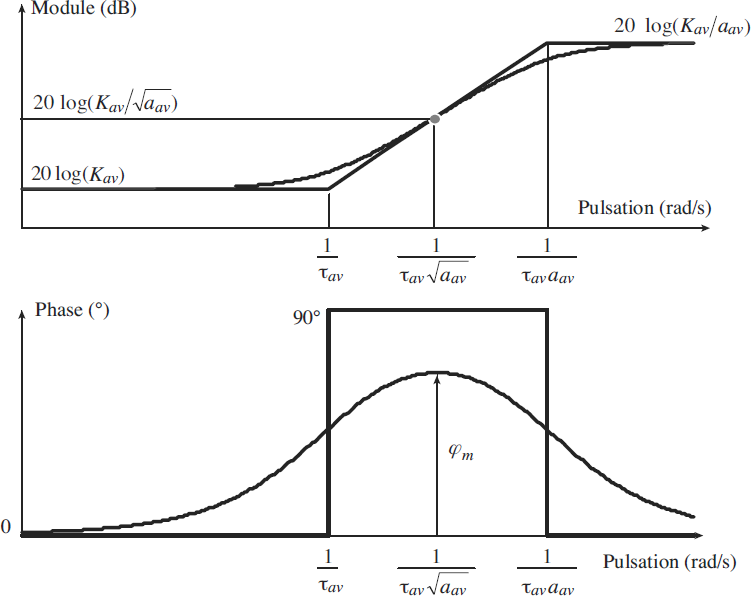
\includegraphics[width=.8\linewidth]{images/pt_15}
\end{center}

\end{minipage}
%%%%%%%%%%%%%%%%%%%%%%%%%%%%%%%%%%%
%%%%%%%%%%%%%%%%%%%%%%%%%%%%%%%%%%%%


\end{multicols}
%
%
%\newpage
%
%\begin{center}
%%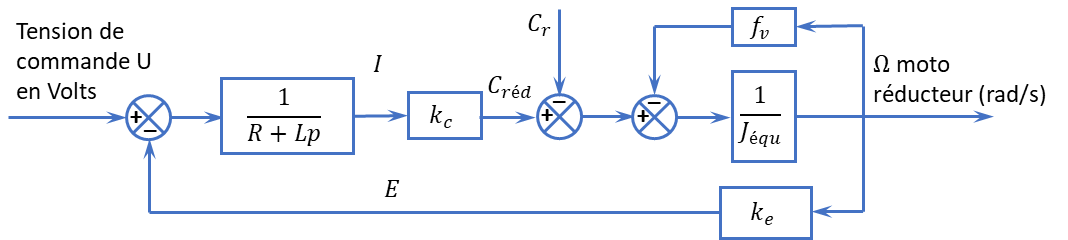
\includegraphics[width=\linewidth]{images/cor_01}
%%\textit{}
%\end{center}
%
%
%\begin{center}
%%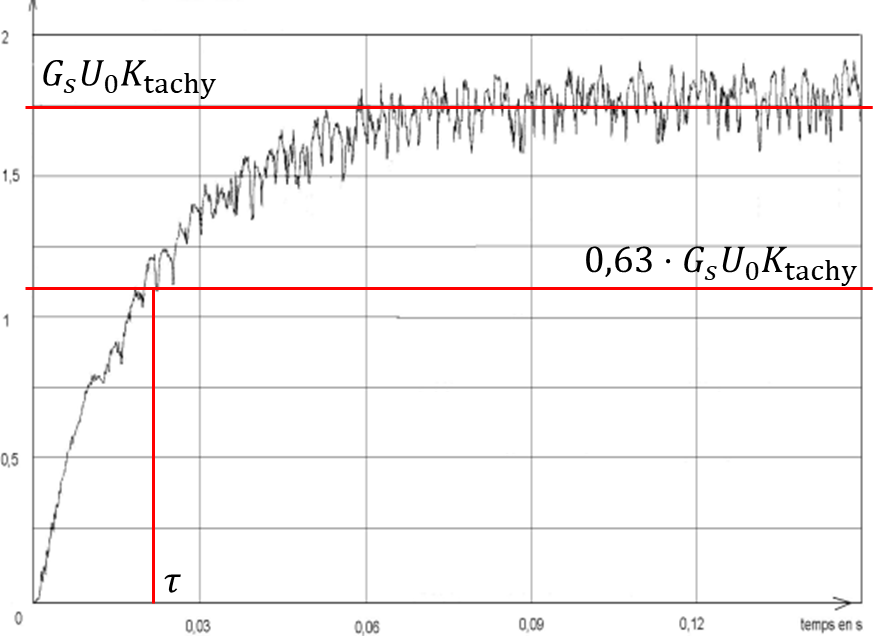
\includegraphics[width=\linewidth]{images/cor_02}
%%\textit{}
%\end{center}


%
%
%\newpage
%
%
%\begin{center}
%	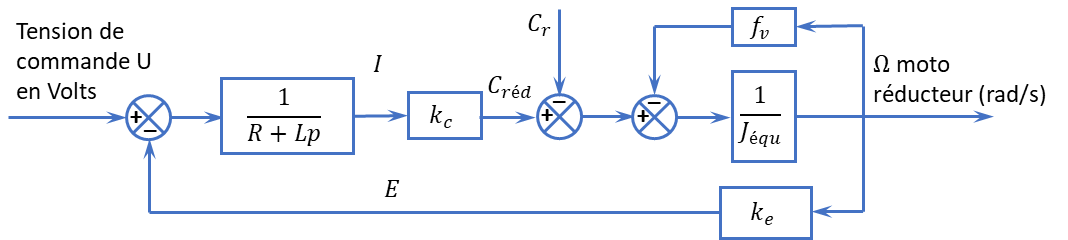
\includegraphics[width=.9\linewidth]{images/cor_01}
%\end{center}
%
%\begin{center}
%	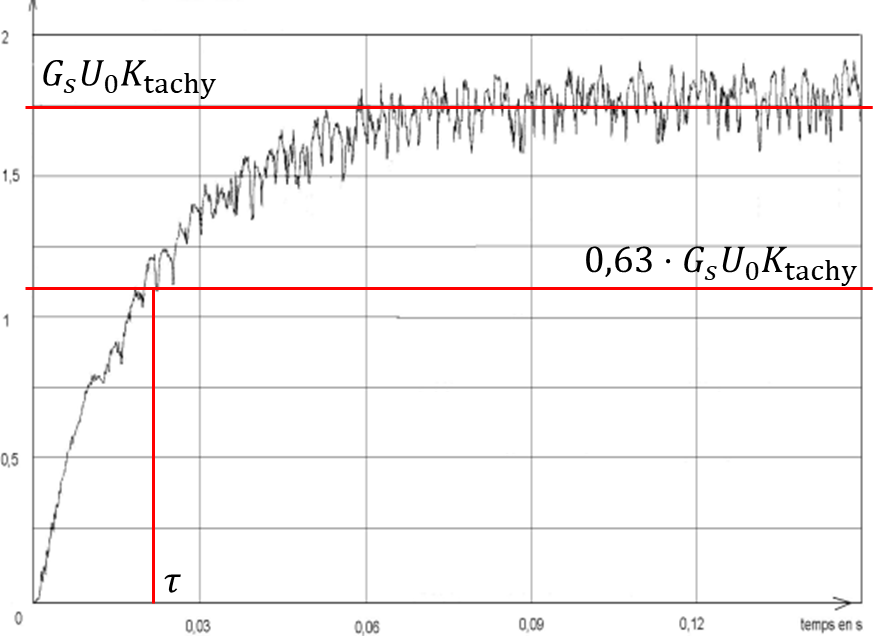
\includegraphics[width=.9\linewidth]{images/cor_02}
%\end{center}
%
%\begin{center}
%	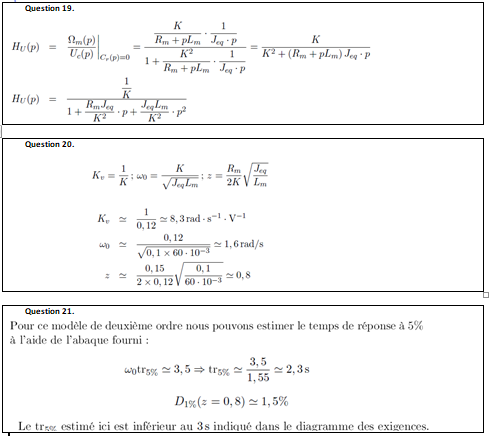
\includegraphics[width=.9\linewidth]{images/cor_03}
%\end{center}
%
%\begin{center}
%	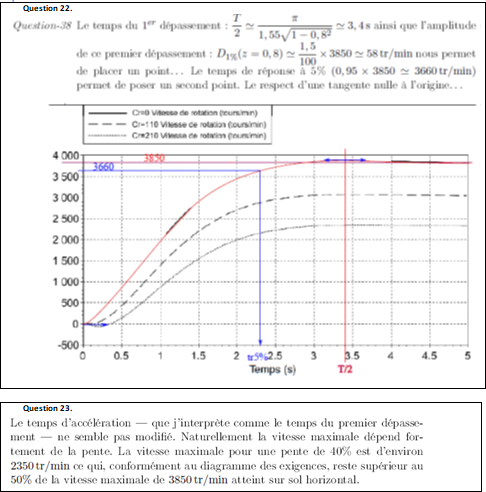
\includegraphics[width=.9\linewidth]{images/cor_04}
%\end{center}

\end{document}

\subparagraph{}\textit{}


\begin{center}
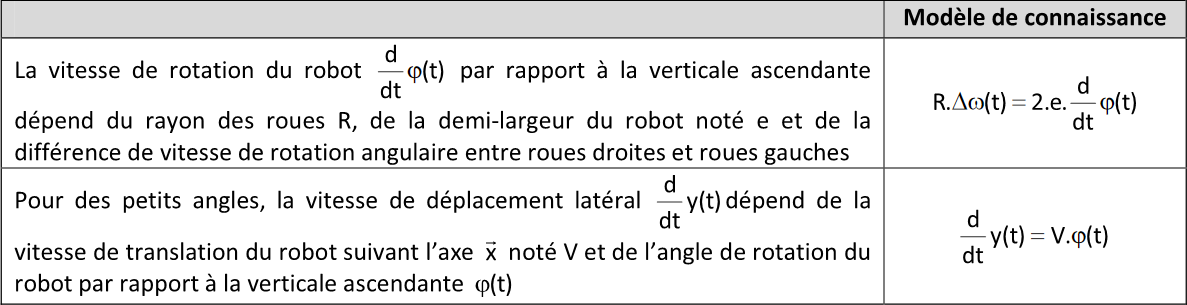
\includegraphics[width=\linewidth]{images/fig_06}
%\textit{}
\end{center}
\begin{center}
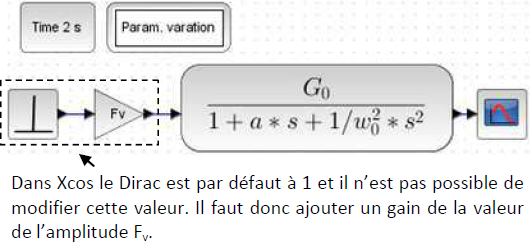
\includegraphics[width=\linewidth]{images/img_04}
%\textit{}
\end{center}

